\part{其他知识}

\chapter{相机、镜头和光场}

\section{小孔成像}

用一个带有小孔的板遮挡在墙体与物之间, 墙体上就会形成物的倒立的实像, 我们把这样的一种现象叫\textbf{小孔成像 (Pinhole Image Formation) }. 小孔成像的特点是得到的成像没有景深效果. 

除了小孔成像之外, 我们还会使用透镜成像. 之所以必须要使用小孔或者透镜是因为传感器上每个点需要记录对应方向光线的数据. 如果不使用小孔或者透镜, 那么到达传感器上的光线将来自各个方向, 不能区分. 

\section{视场}

摄像机的\textbf{视场 (Field of View, FOV) }的大小和传感器的大小以及焦距 (小孔成像中指的是传感器和小孔的距离) 有关. 

\begin{figure}[H]
	\centering
	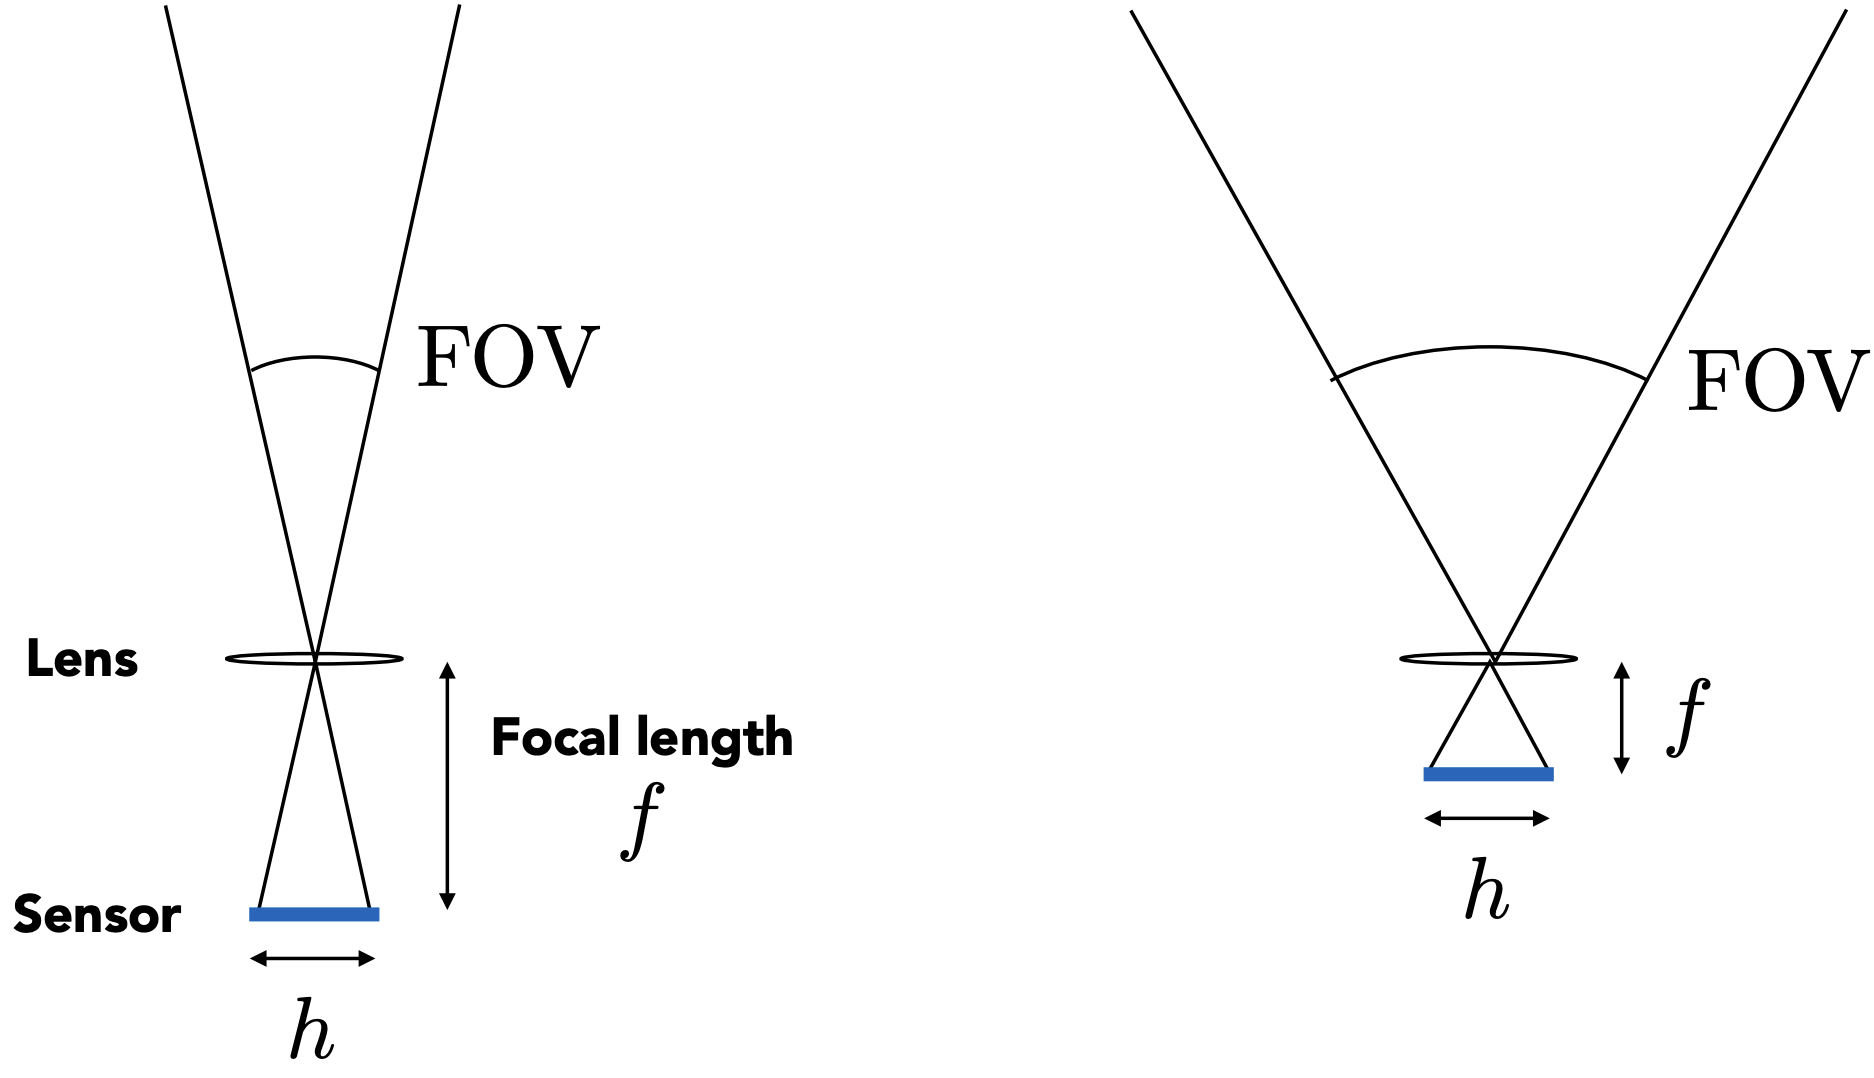
\includegraphics[scale=.25]{fov.png}
	\caption{FOV}
	\label{fig:fov}
\end{figure}

根据相似三角形性质可知, 
\begin{equation}
	\text{FOV}=2\arctan(\frac{h}{2f})
\end{equation}

\begin{itemize}
	\item 传感器越大, 视场越大; 
	\item 焦距越短, 视场越大. 
\end{itemize}

由于一些历史原因, 在实际应用中, 我们会采用35mm胶片 ($36\times 24 mm$) 对应的焦距来反映视场的大小. 焦距越小, 对应的视场越大; 焦距越大, 拍摄的距离越远. 较小的传感器需要使用较短的焦距来保持一样的视场. 

\section{曝光}

\textbf{曝光 (Exposure, $H$) }可以表示为曝光时间$T$和Irradiance $E$的乘积. 
\begin{equation}
	H=T\times E
\end{equation}
其中, 曝光时间由快门控制, Irradiance是单位时间传感器单位面积上接受的光的强度, 由光圈和焦距控制. 

\subsection{曝光控制}

曝光的控制由以下三个参数决定: 
\begin{itemize}
	\item 光圈大小 (Aperture Size) : 光圈的大小由f-stop控制, 光圈是一个类似于瞳孔的结构. 记做$FN$或者$F/N$, 其中$N$是f数, 计算方法是$f/D$, 也就是焦距除以光圈的直径. 光圈越大, 景深效果越明显. 
	\item 快门速度 (Shutter Speed ) : 决定了传感器的感光时间; 快门速度越慢, 得到的图片会出现模糊, 我们称作\textbf{运动模糊 (Motion Blur) }. 运动模糊会使图像变模糊, 但是可以体现出运动速度快, 符合人眼规律. 对于某些包含快速旋转物体的图片, 由于图像每一个部分都在不同时间拍摄, 因此会出现\textbf{卷帘快门 (Rolling Shutter) }的现象. 
	\item ISO感光度 (ISO Gain) : 传感器值乘一个常数变换为数字图像值, 是一种后期处理. 在数字相机中, 高ISO会增加噪声. ISO是一种线性增长 (ISO 200增加亮度的一半就是ISO 100) . 
\end{itemize}

\begin{figure}[H]
	\centering
	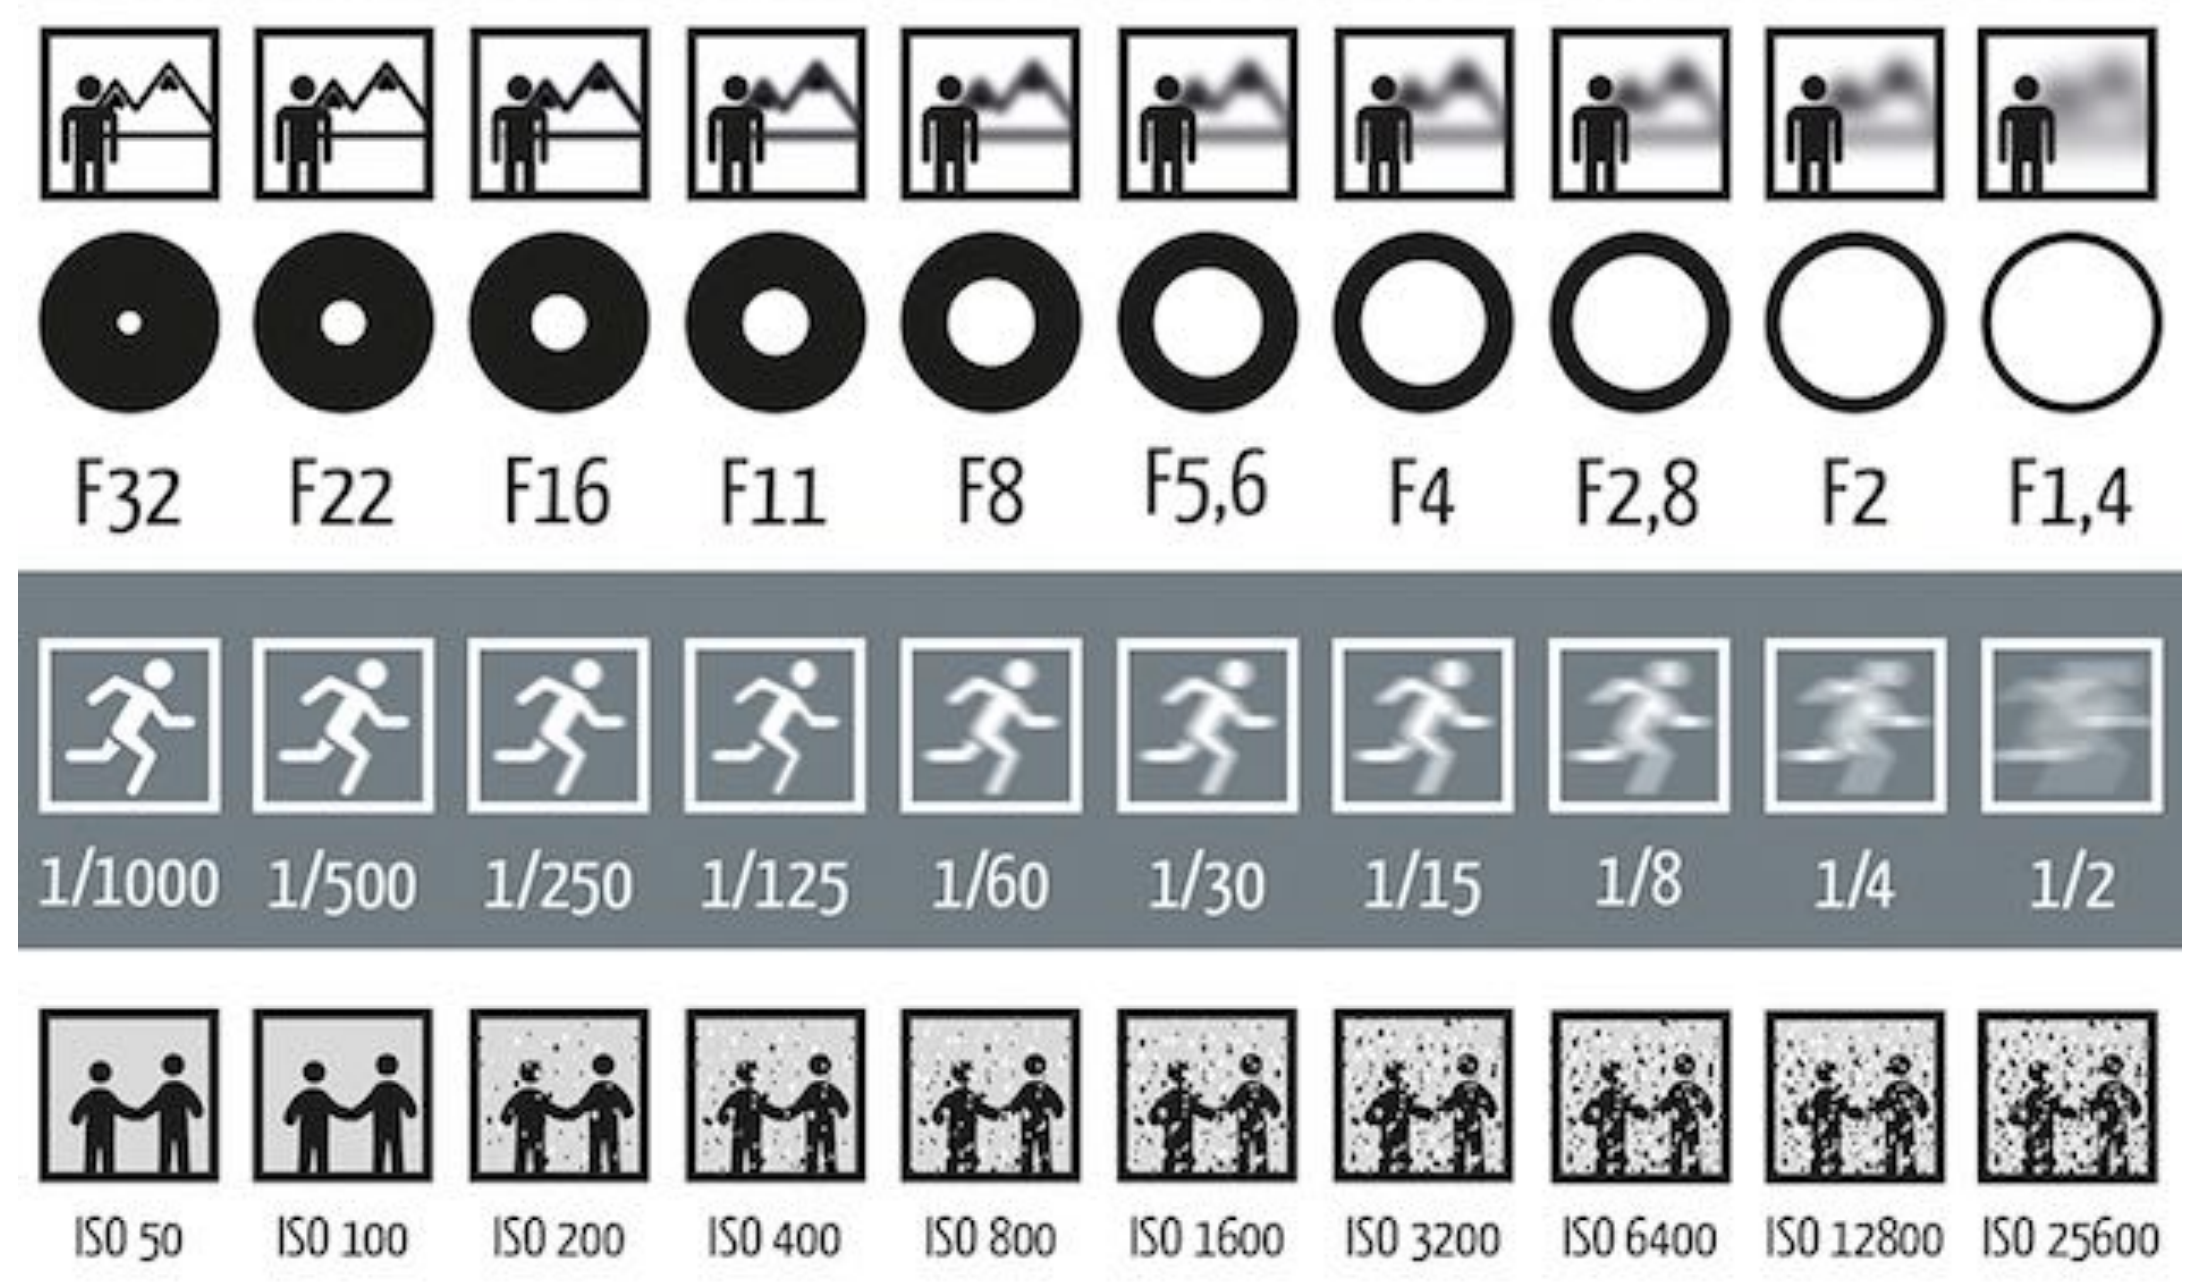
\includegraphics[scale=.25]{expose.png}
	\caption{常见曝光参数的比较}
	\label{fig:expose}
\end{figure}

光圈和快门速度都可以控制曝光, 因此理论上在一定的组合方式下, 能够得到相同的曝光结果. 但是, 由于光圈和快门速度所带来的副作用不同, 因此不同组合产生的效果也会有一些不同. 在下表中, 光圈和快门速度的组合能够得到相同的曝光. 

\begin{table}[H]
	\centering
	\begin{tabular}{ccccccccccc}
		\hline
		f-stop & 1.4   & 2.0   & 2.8   & 4.0  & 5.6  & 8.0  & 11.0 & 16.0 & 22.0 & 32.0 \\
		快门速度   & 1/500 & 1/250 & 1/125 & 1/60 & 1/30 & 1/15 & 1/8  & 1/4  & 1/2  & 1 \\	\hline
	\end{tabular}
	\caption{光圈和快门速度组合表, 以上组合得到的曝光理论一致}
\end{table}

\section{薄透镜近似 (Thin Lens Approximation) }

真实的透镜都是由透镜组所组成的. 真实的透镜并不是理想的, 这是因为平行光经过真实透镜后不能聚焦在同一个点上. 理想的薄透镜满足以下三点: 
\begin{enumerate}
	\item 所有经过透镜的平行光都会聚焦在它的焦点; 
	\item 所有经过透镜的焦点的光都会变成平行光; 
	\item 透镜的焦距可以任意的变换. 
\end{enumerate}

\subsection{透镜方程}

在薄透镜中, 焦距$f$, 物距$z_o$, 像距$z_i$满足
\begin{equation}
	\frac{1}{f}=\frac{1}{z_o}+\frac{1}{z_i}
\end{equation}

这被称为\textbf{薄透镜方程 (The Thin Lens Equation) }. 

\begin{figure}[H]
	\centering
	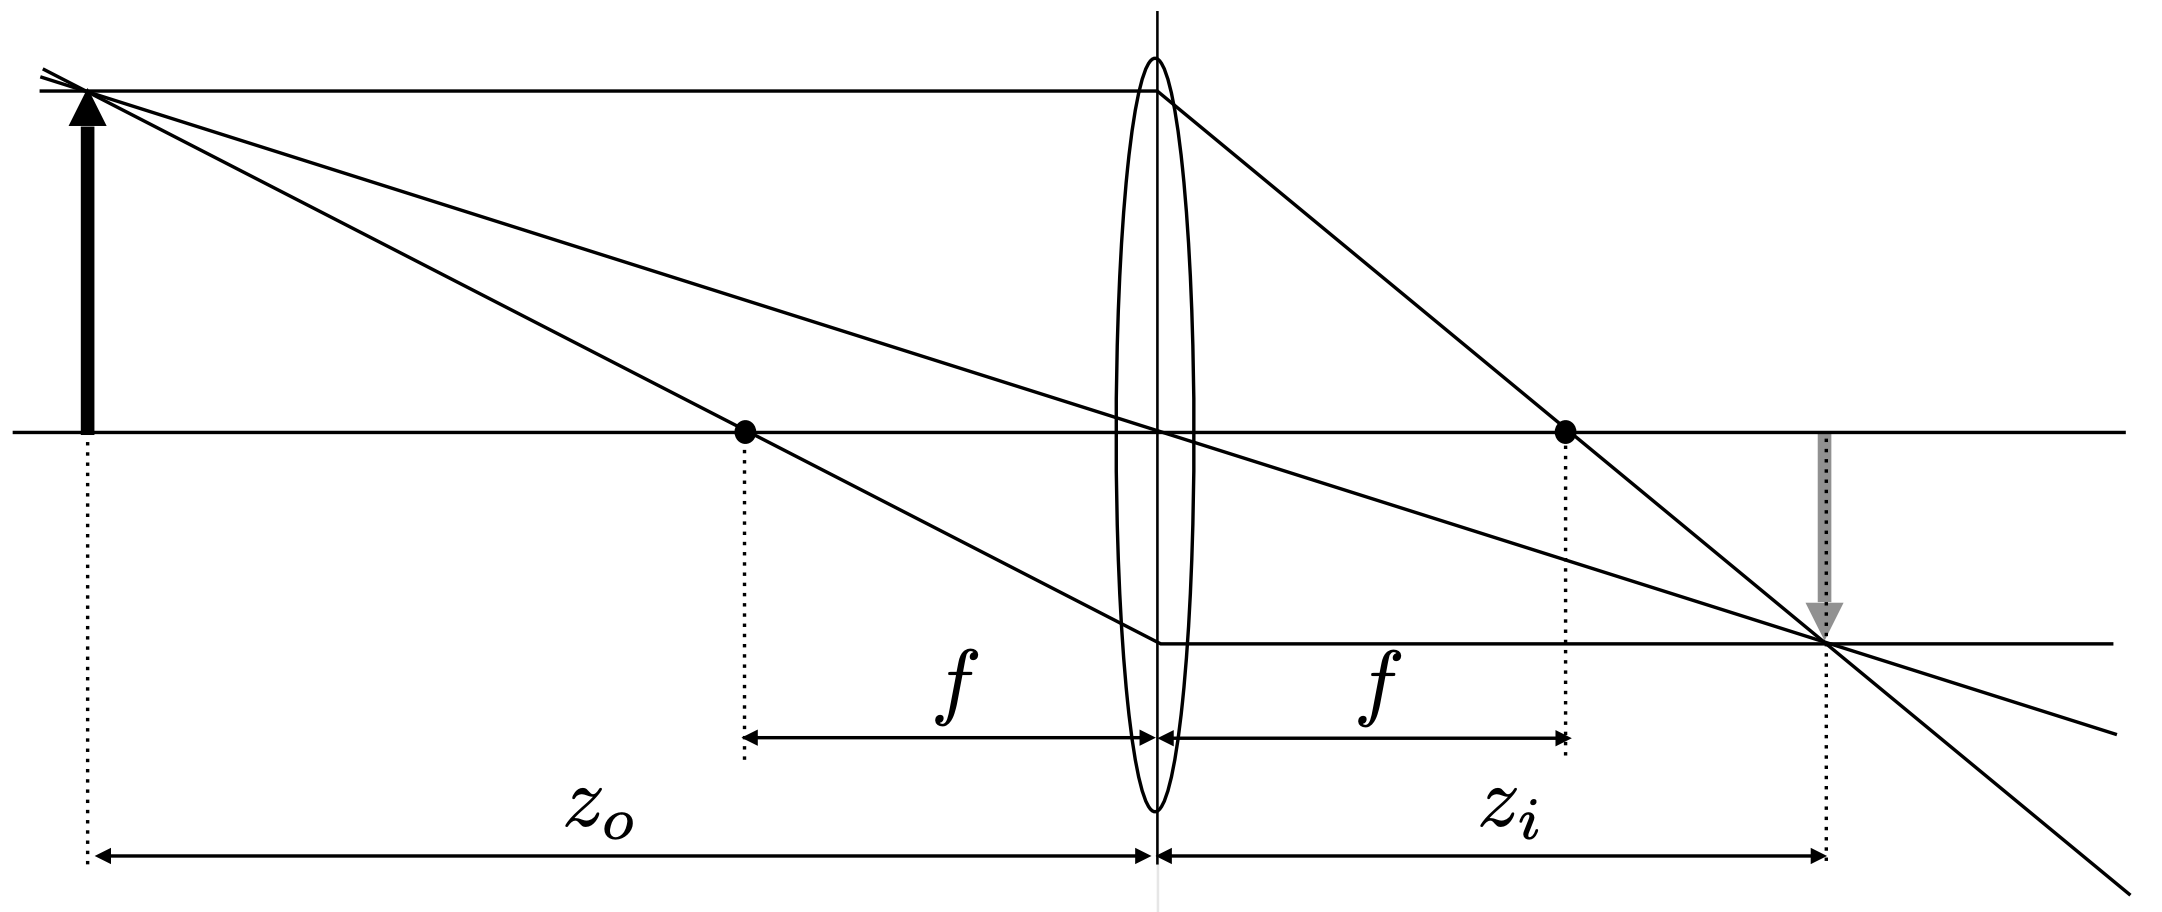
\includegraphics[scale=.20]{lenequ.png}
	\caption{透镜光学传播示意图}
	\label{fig:lenequ}
\end{figure}

\begin{titledbox}{薄透镜方程的证明}
	
	\begin{figure}[H]
		\centering
		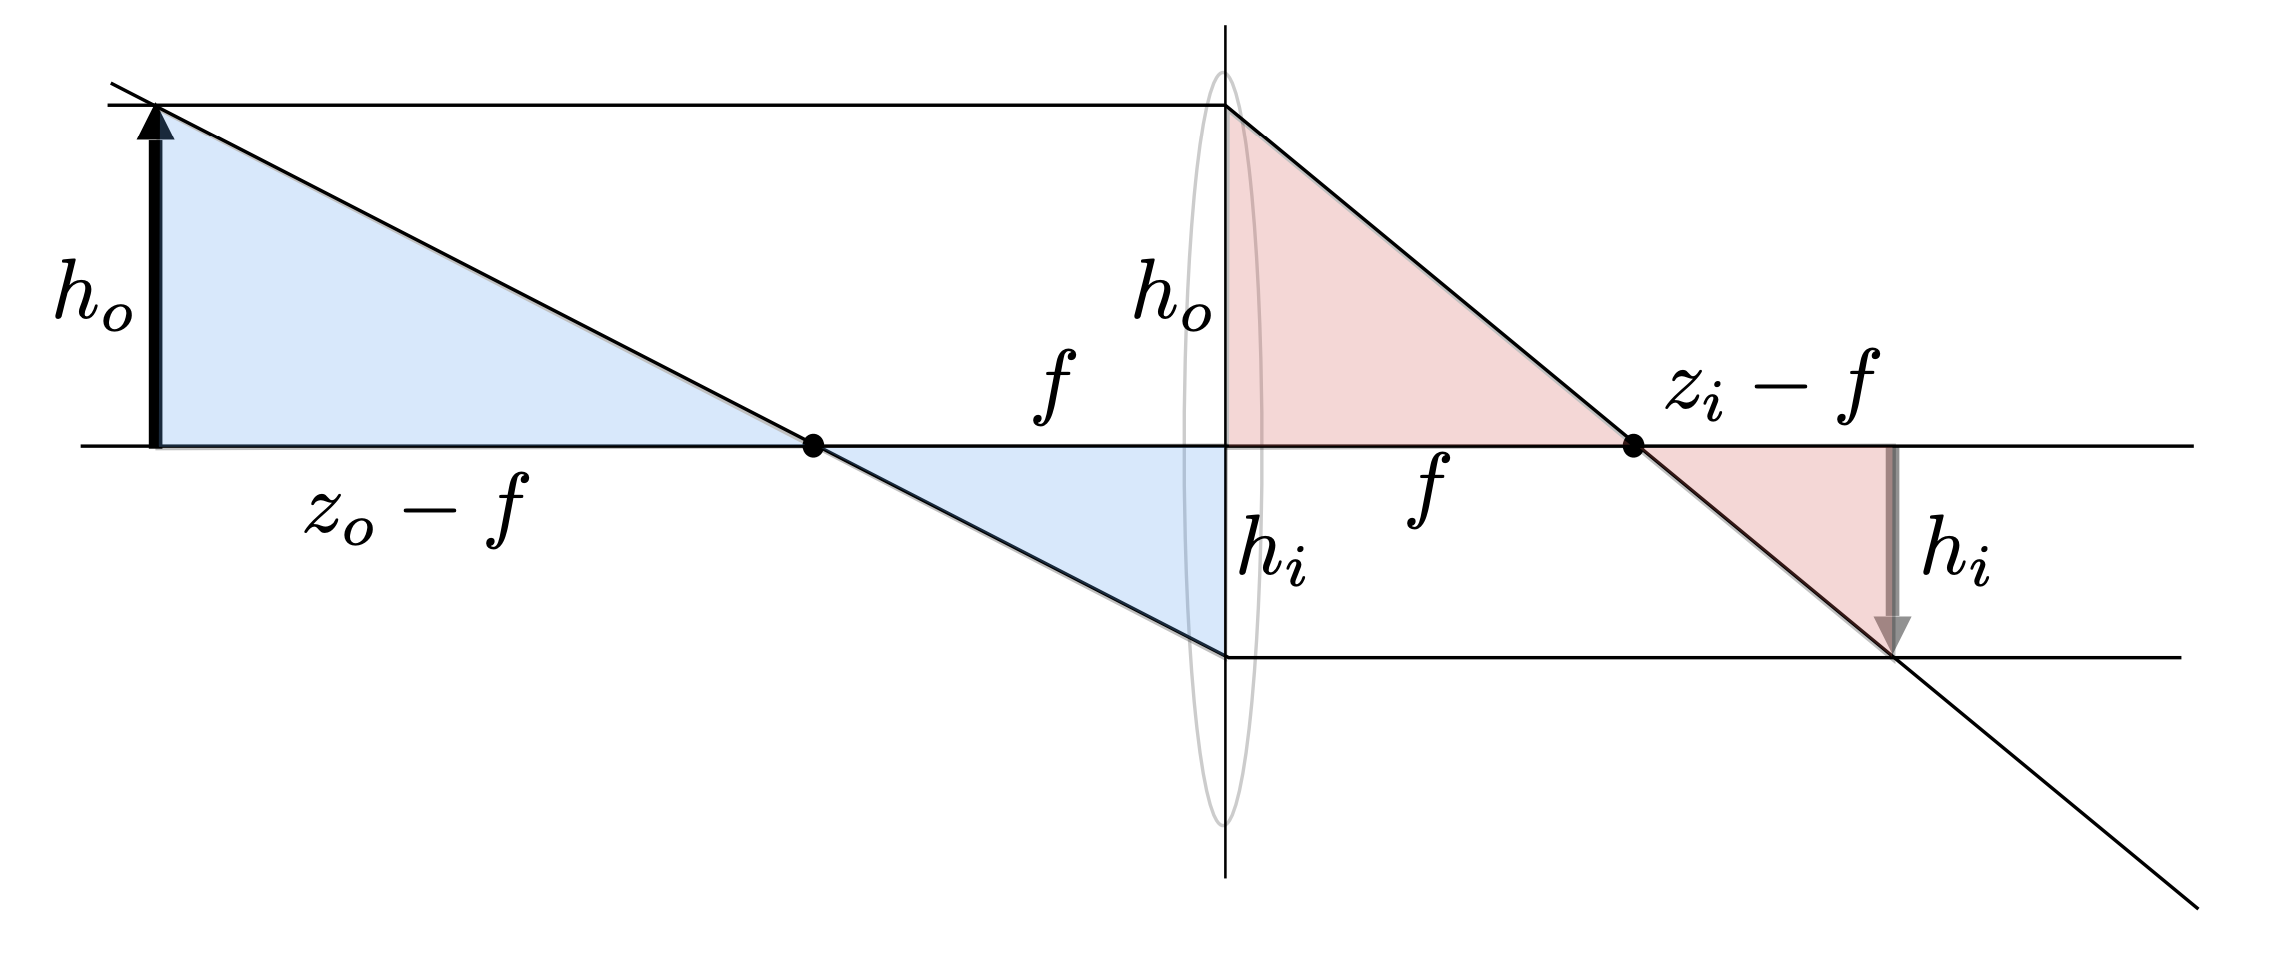
\includegraphics[scale=.20]{lenequz.png}
		\caption{薄透镜方程的证明}
		\label{fig:lenequz}
	\end{figure}

根据相似三角形的性质, 我们可以从蓝色相似三角形组和红色相似三角形组可以得到: 
\begin{equation}
	\begin{split}
		\frac{h_o}{z-f}&=\frac{h_i}{f}\\
		\frac{h_o}{f}&=\frac{h_i}{z_i-f}
	\end{split}
\end{equation}

联立公式可以得到: 
\begin{equation}
	\frac{z_o-f}{f}=\frac{f}{z_i-f}
\end{equation}

整理可得

\begin{equation}
	\frac{1}{f}=\frac{1}{z_o}+\frac{1}{z_i}
\end{equation}
	
\end{titledbox}

\subsection{离焦模糊}

当我们的物体不在聚焦平面的时候, 它的像对应在传感器平面上是一个光圈, 这个光圈被称为\textbf{弥散圆 (Circle of Confusion,  CoC) }. 因此当物体不在聚焦平面上的时候, 会产生一个模糊的光圈, 这就是\textbf{离焦模糊 (Defocus Blur) }现象. 

	\begin{figure}[H]
	\centering
	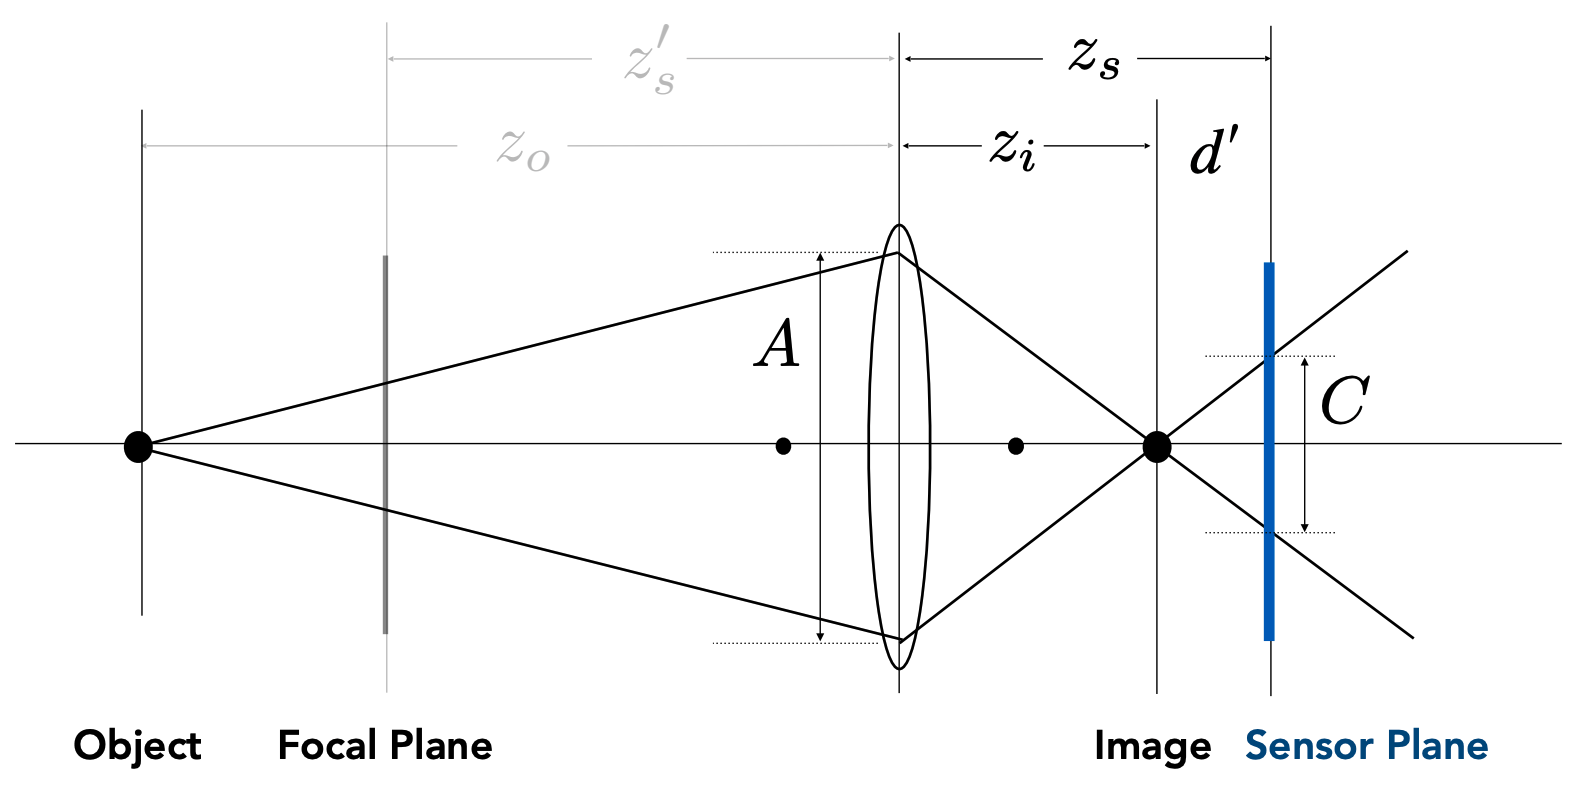
\includegraphics[scale=.15]{coc.png}
	\caption{弥散圆}
	\label{fig:coc}
\end{figure}

弥散圆的直径$C$和透镜的直径$A$满足: 
\begin{equation}
	\frac{C}{A}=\frac{d'}{z_i}=\frac{|z_s-z_i|}{z_i}
\end{equation}

我们又知道, 光圈的大小f-stop由焦距和光圈的直径有决定. 因此, 上式可以改写成: 
\begin{equation}
	C=A\frac{|z_s-z_i|}{z_i}=\frac{f}{N}\frac{|z_s-z_i|}{z_i}
\end{equation}

因此, 光圈f-stop越大, 拍出来的相片越清晰, 对应光圈的直径越小. 

\subsection{薄透镜下的光线追踪}

	\begin{figure}[H]
	\centering
	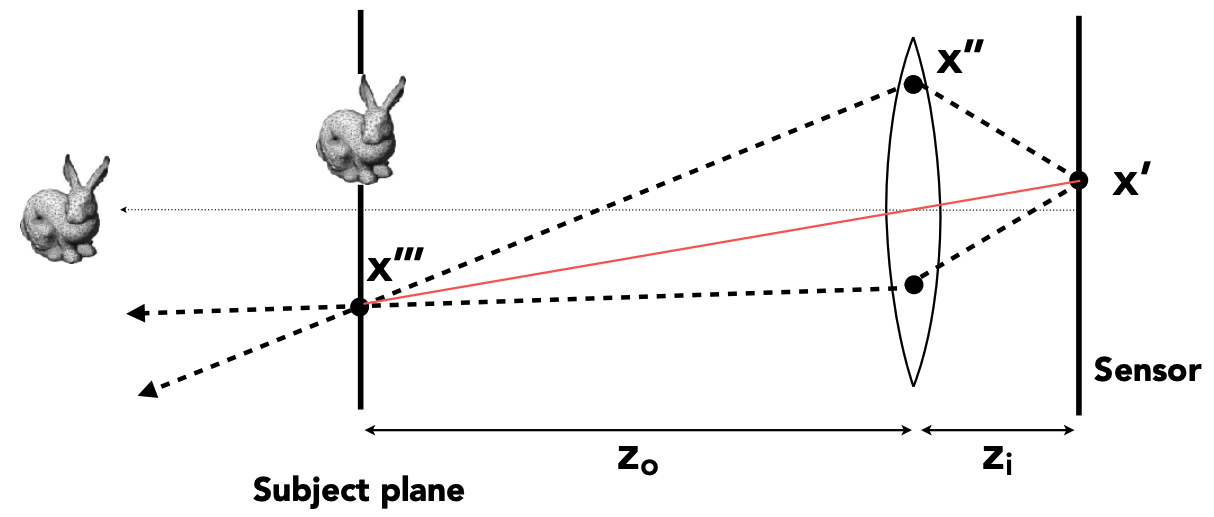
\includegraphics[scale=.20]{raylen.png}
	\caption{薄透镜下的光线追踪}
	\label{fig:raylen}
	\end{figure}

之前我们的路径追踪都是在小孔摄像机的假设下. 现在我们使用薄透镜模型进行光线追踪. 首先, 我们需要定义
\begin{itemize}
	\item 传感器大小, 透镜的焦距以及透镜的孔径大小; 
	\item 确定成像平面的距离$z_o$. 那么我们可以推算出传感器平面的距离$z_i$. 
\end{itemize}

我们按照以下方法确定路径: 
\begin{itemize}
	\item 选定每一个传感器像素上的点$x'$; 
	\item 在透镜平面上随机采样点$x''$; 
	\item 光线经过透镜会打到成像平面上的$x'''$点; 
	\item 计算从$x'''$到$x''$的radiance, 就是对应$x'$的结果. 
\end{itemize}

\subsection{景深}

	我们认为, 当一段深度的物体能够保证CoC是足够小的, 那么这一段深度我们称作\textbf{景深 (Depth of Field) }. 在实际中我们认为CoC小于一个像素的大小都可以看作足够小. 景深的计算如下所示: 
	
		\begin{figure}[H]
		\centering
		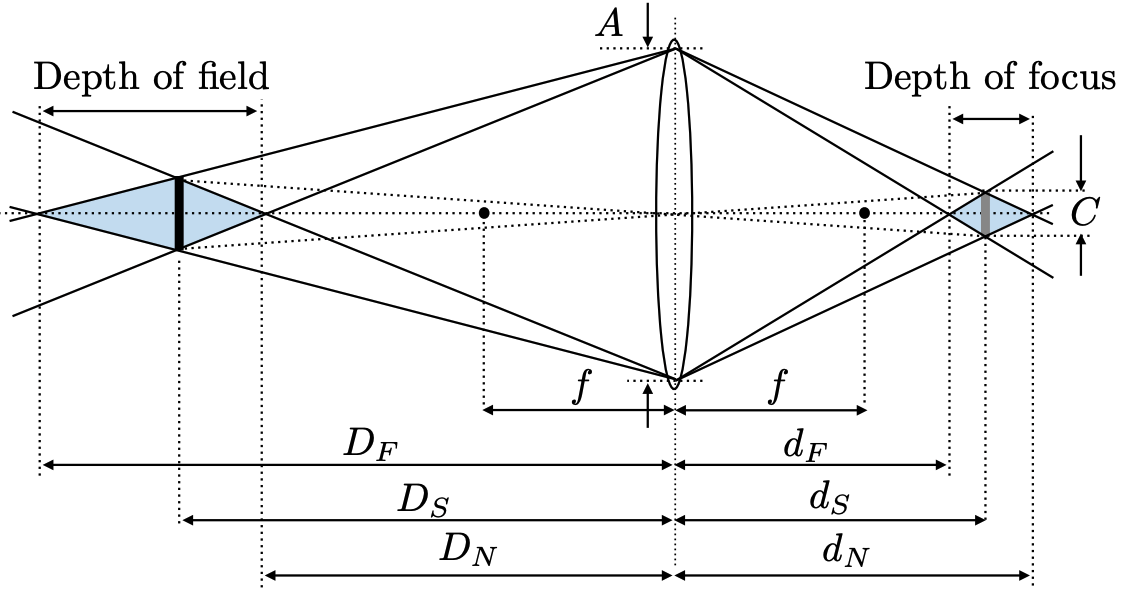
\includegraphics[scale=.20]{dof.png}
		\caption{景深的计算}
		\label{fig:dof}
	\end{figure}

根据离焦模糊公式和薄透镜方程有: 
\begin{equation}
	\begin{split}
		\frac{d_{N}-d_{S}}{d_{N}} &=\frac{C}{A} \\
		\frac{d_{S}-d_{F}}{d_{F}} &=\frac{C}{A} \\
		N &=\frac{f}{A} \\
		\frac{1}{D_{F}}+\frac{1}{d_{F}} &=\frac{1}{f} \\
		\frac{1}{D_{S}}+\frac{1}{d_{S}} &=\frac{1}{f} \\
		\frac{1}{D_{N}}+\frac{1}{d_{N}} &=\frac{1}{f}
	\end{split}
\end{equation}

因此: 
\begin{equation}
	\begin{split}
		\mathrm{DOF}&=D_{F}-D_{N} \\
		D_{F}&=\frac{D_{S} f^{2}}{f^{2}-N C\left(D_{S}-f\right)}\\
		D_{N}&=\frac{D_{S} f^{2}}{f^{2}+N C\left(D_{S}-f\right)}
	\end{split}
\end{equation}

\section{光场}

对于人眼来说, 不关心光线究竟是从哪里来的. 因此我们可以用一张图片来模拟一种光. 在这里我们提出\textbf{全光函数 (The Plenoptic Function) }. 我们的视觉世界可以使用7个维度描述: 
\begin{equation}
	P(\theta,\phi,\lambda,t,V_X,V_Y,V_Z)
\end{equation}

\begin{itemize}
	\item $\theta,\phi$是立体角变量, 通过这两个参数可以描述光线的强度 (也就是灰度值) ; 
	\item $\lambda$代表不同的波长, 可以描述颜色信息; 
	\item $t$, 时间维度, 这可以看作电影; 
	\item $V_X,V_Y,V_Z$, 位置函数, 可以看作全息电影. 
\end{itemize}

通过全光函数, 我们可以记录所有的信息. \textbf{光场 (Light Field / Lumigraph) }可以看作全光函数的一部分信息. 

首先, 我们定义光线, 我们忽略颜色和时间参数. 光线可以由两种方式进行定义, 第一种方式是使用3维的起点以及2维的方向定义光线: 
\begin{equation}
	P(\theta,\phi,V_X,V_Y,V_Z)
\end{equation}

通过5个维度我们定义了一个光线. 但是我们可以通过两个点定义一条光线, 这样子我们只需要四个维度就可以表示一条光线 (只要我们定义好两个平面, 上面的点都是2维的, 因此两个点只需要4个维度就可以了) . 

对于任何一个物体, 我们可以使用一个包围盒来描述在各个方向上看到的光线情况. 我们不关心包围盒内的物体情况, 我们在观察时只用查询对应光场函数就可以了. 

\begin{figure}[H]
	\centering
	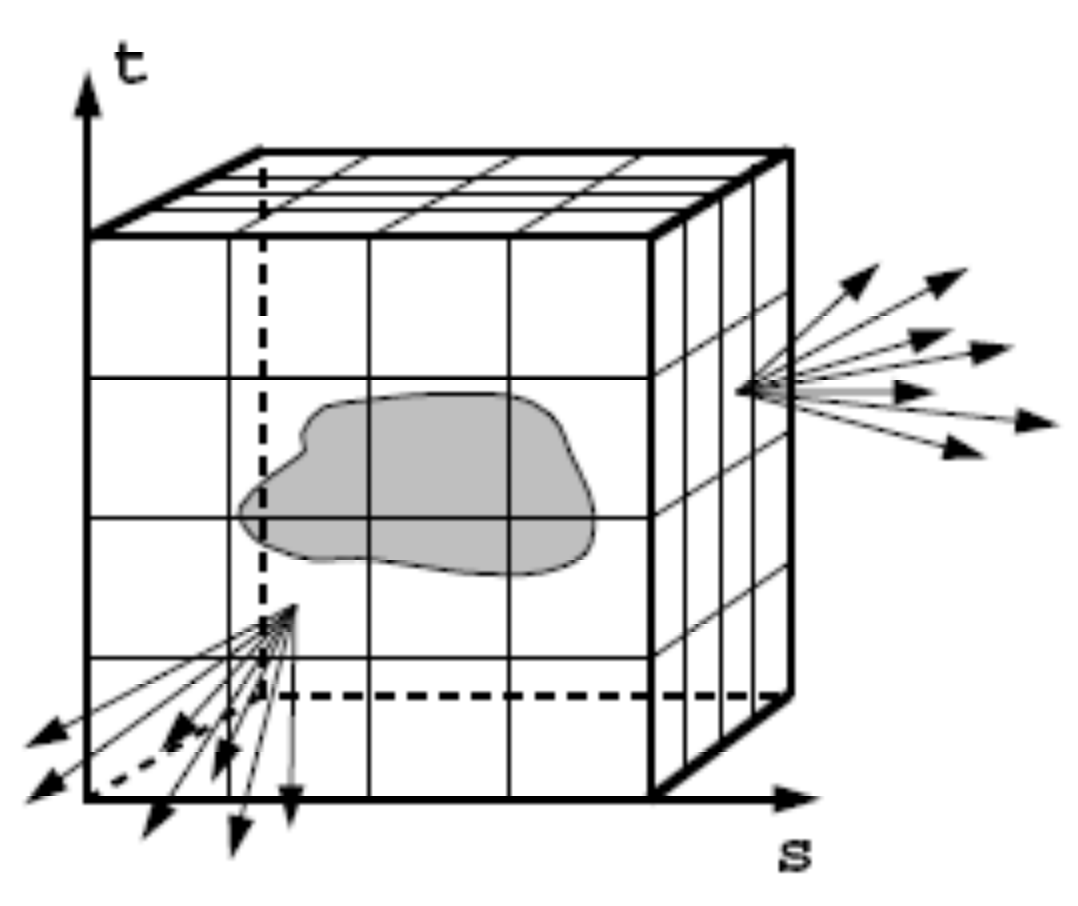
\includegraphics[scale=.20]{guangchang.png}
	\caption{包围盒的光场}
	\label{fig:guangchang}
\end{figure}

我们关注一个面上的光场情况. 前文提到, 我们可以使用两个点表示一条光线. 因此对于光场, 我们也可以使用两个平面表示一个光场. 其中, 远离物体的为s-t平面, 靠近物体的为u-v平面. 

\begin{figure}[H]
	\centering
	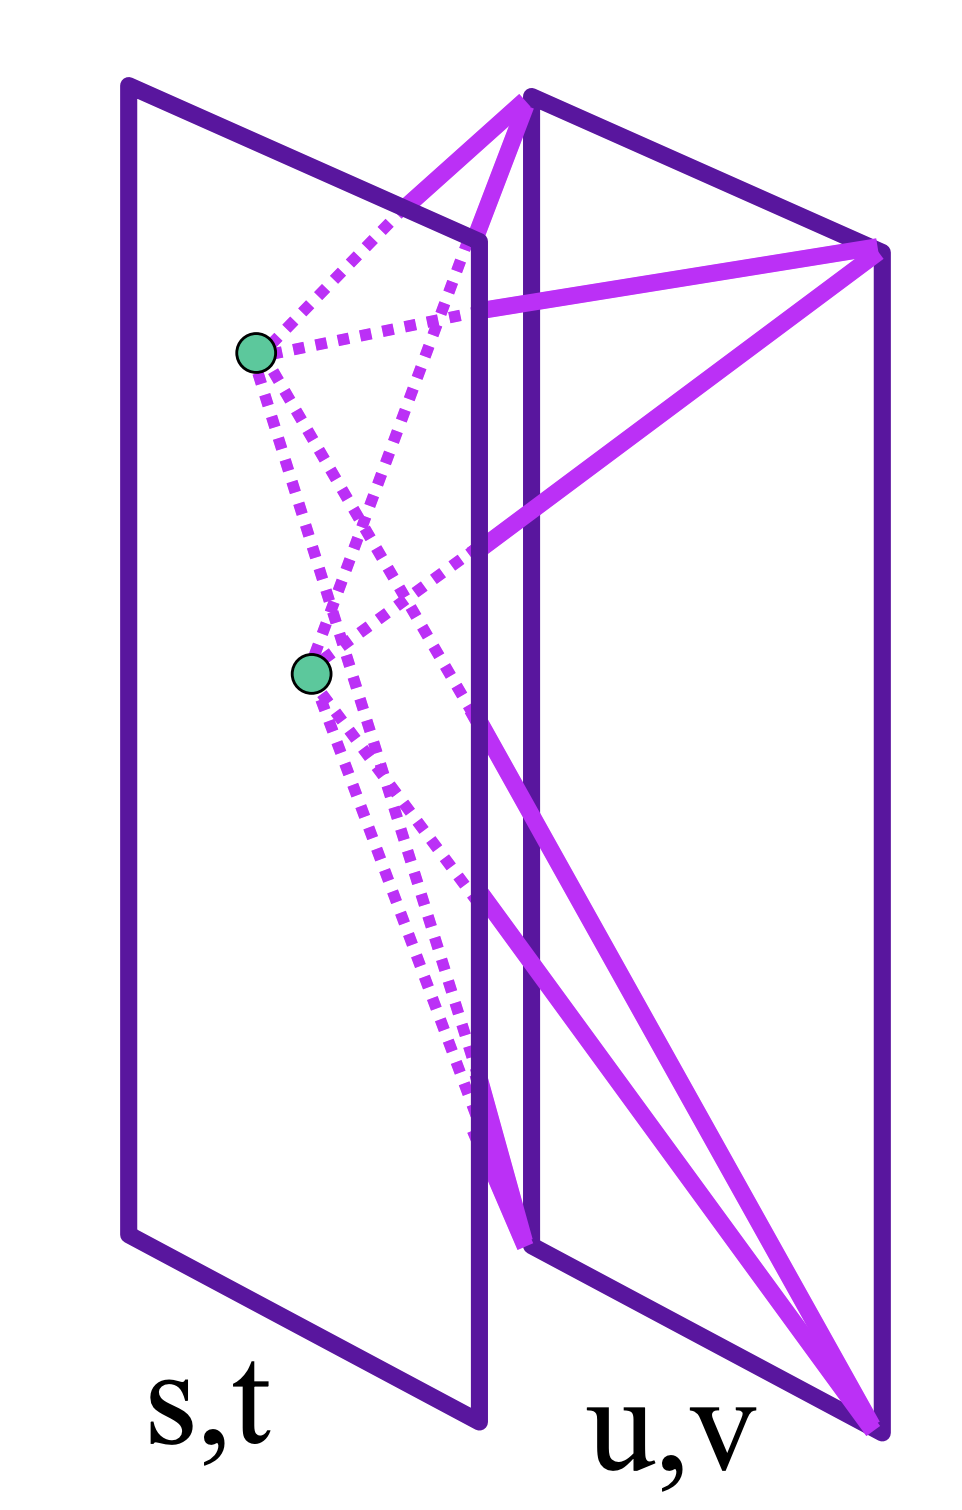
\includegraphics[scale=.15]{stuv.png}
	\caption{使用两个平面表示一个光场}
	\label{fig:stuv}
\end{figure}

如果我们固定某一个平面上面的点, 我们可以观察在另一平面上不同点的分布: 

\begin{figure}[H]
	\centering
	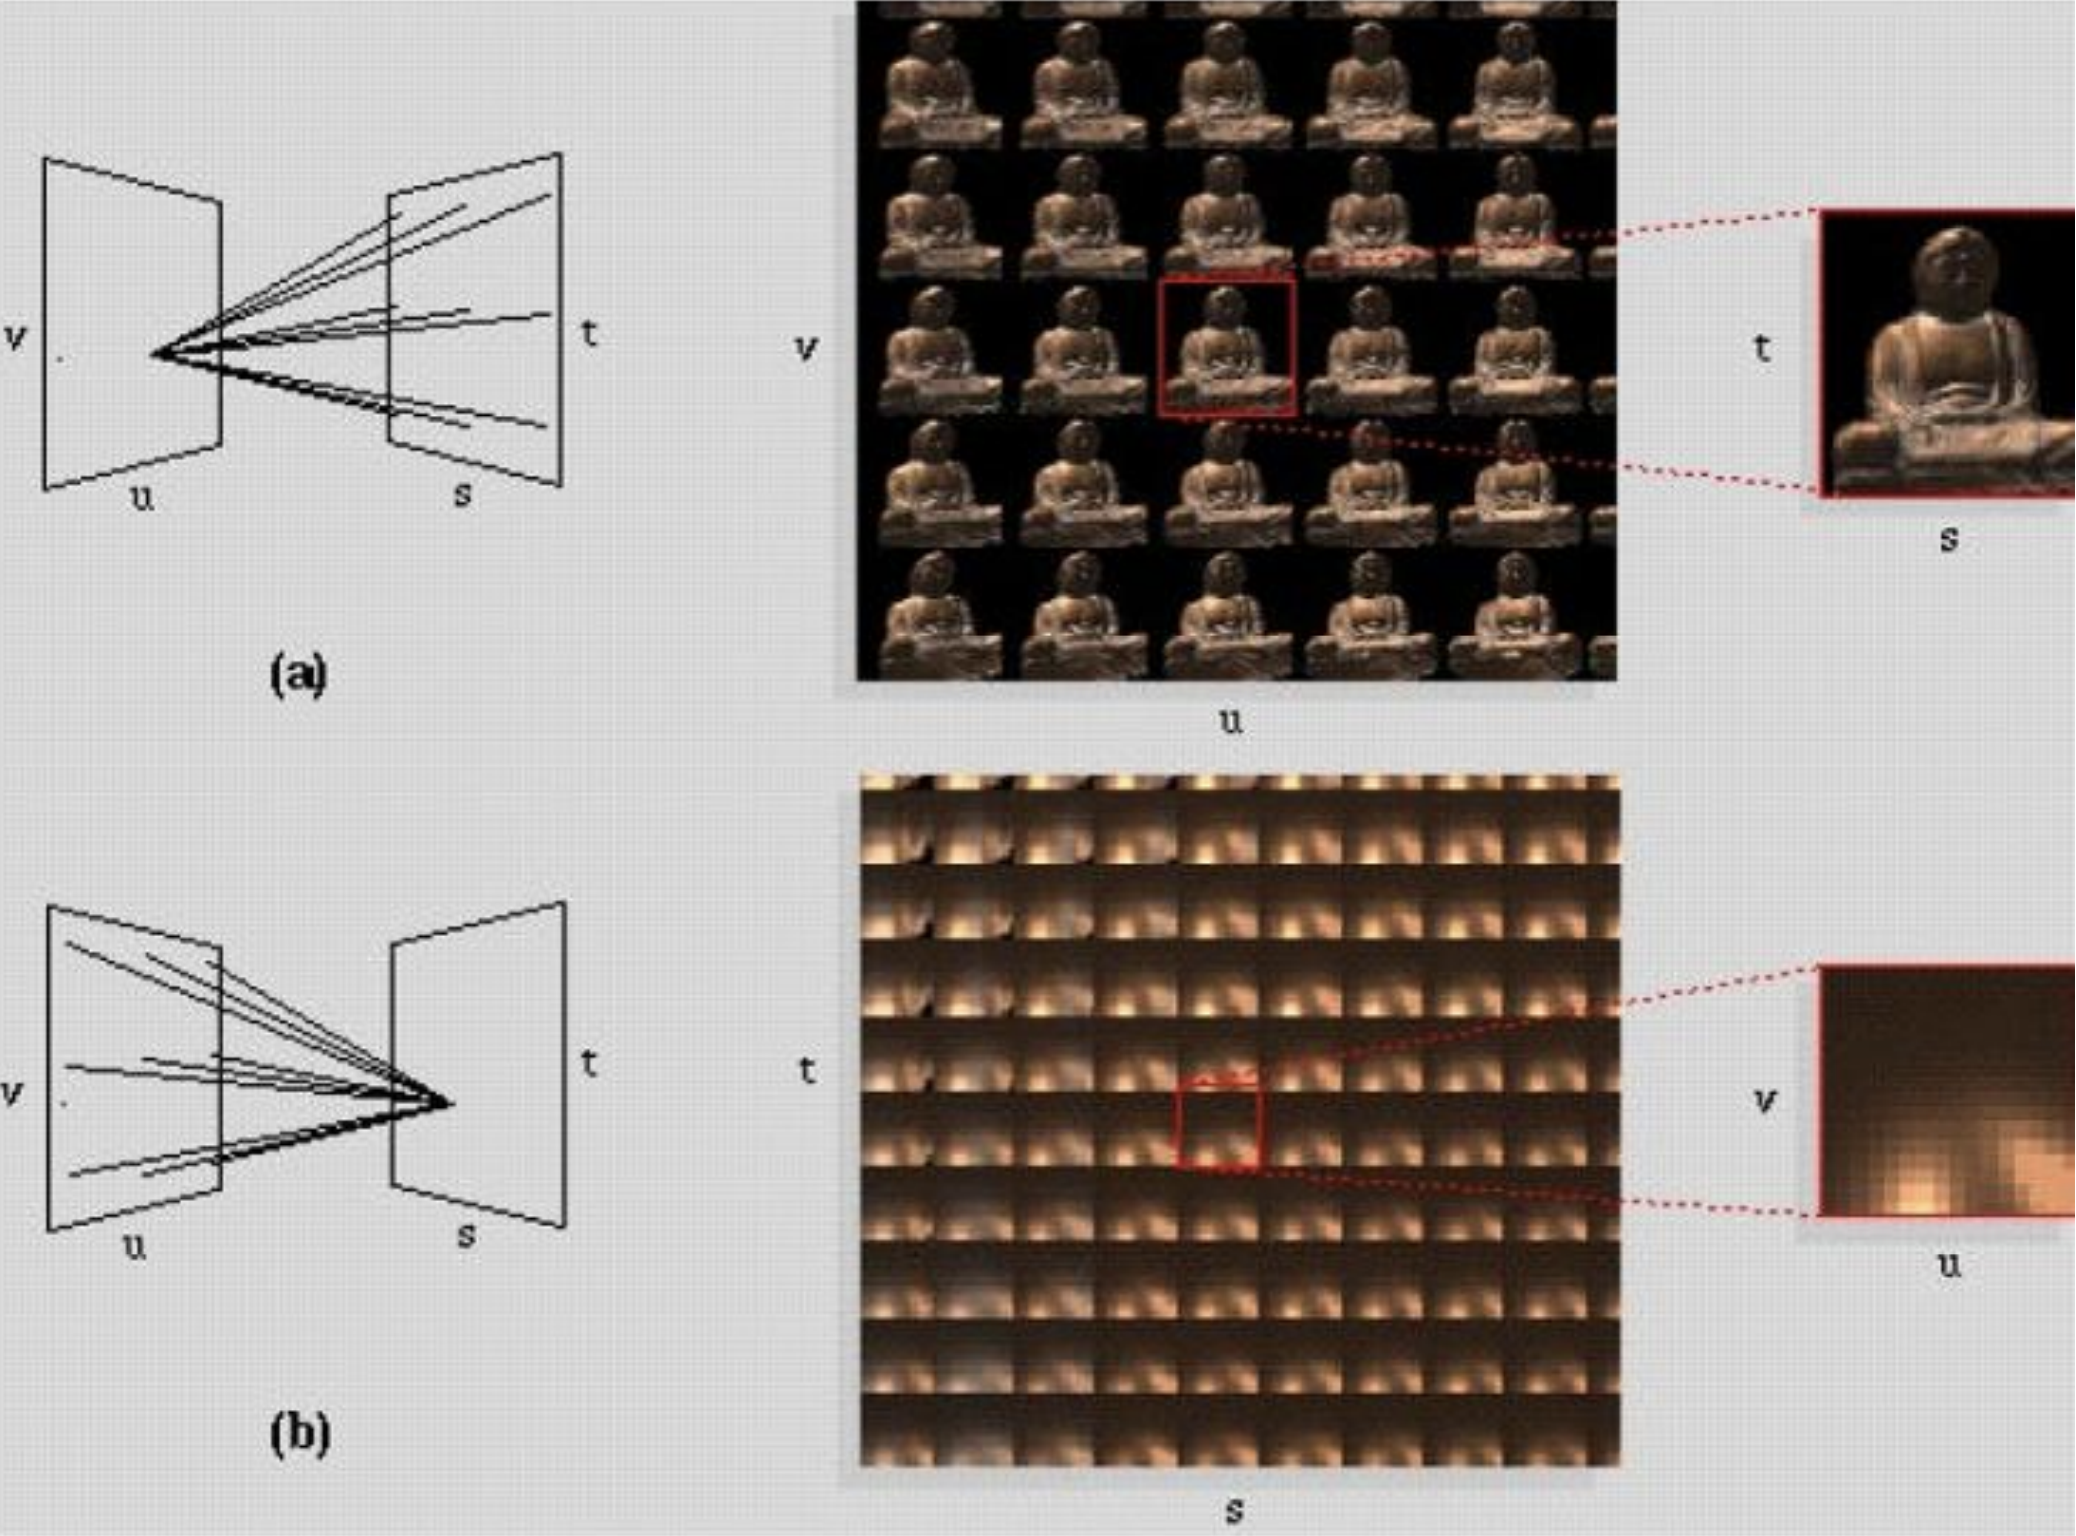
\includegraphics[scale=.3]{stuvkeshi.png}
	\caption{不同平面上表示的内容}
	\label{fig:stuvkeshi}
\end{figure}

\begin{itemize}
	\item 当我们固定u-v平面上的点, 每一个s-t平面都是一副完整的图像; 
	\item 当我们固定s-t平面上的点, 每一个u-v平面上的点都是同一个像素在不同方向上看到的结果. 
\end{itemize}

根据这样的方式, 我们可以造出\textbf{光场照相机 (Light Field Camera) }. 光场照相机是一系列镜头矩阵构成的照相机. 

\begin{figure}[H]
	\centering
	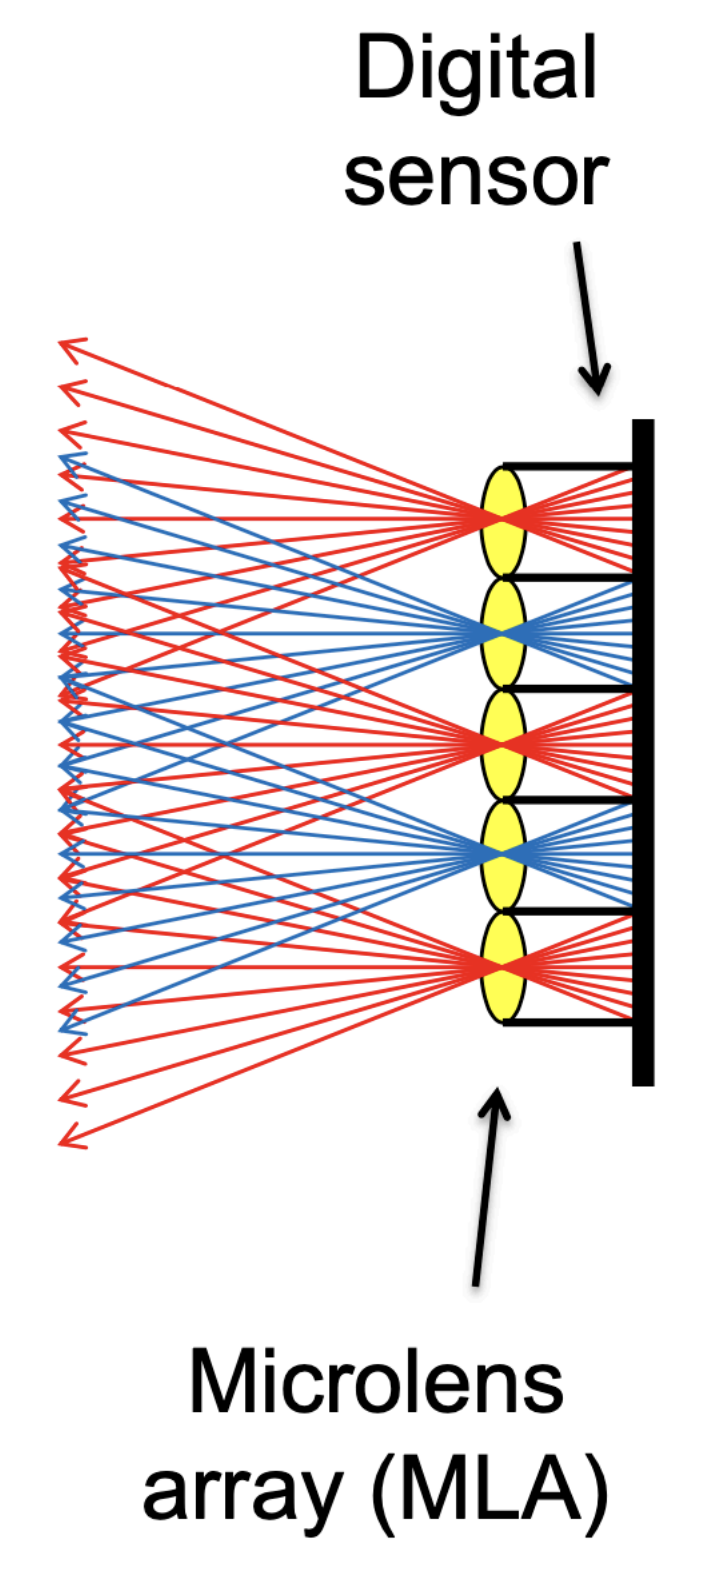
\includegraphics[scale=.2]{guangchangzhaoxiang.png}
	\caption{光场照相机图示}
	\label{fig:guangchangzhaoxiang}
\end{figure}

光场照相机每一个像素点都记录了该点所有方向的光场信息, 因此使用光场照相机可以: 
\begin{itemize}
	\item 在后期方便的移动摄像机的位置; 
	\item 在后期进行对焦. 
\end{itemize}

但是会有成本过高以及分辨率不足的缺点. 

\chapter{颜色}

牛顿通过实验认识到, 白光是由多种颜色的光线混合起来得到的. 而我们在生活中可以看到的光在波长约400mm-700mm之间. 对于不同光, 我们可以使用\textbf{功率谱密度 (Spectral Power Distribution, SPD) }表示. 功率谱密度展示了不同波长下光能量的多少. 

\begin{figure}[H]
	\centering
	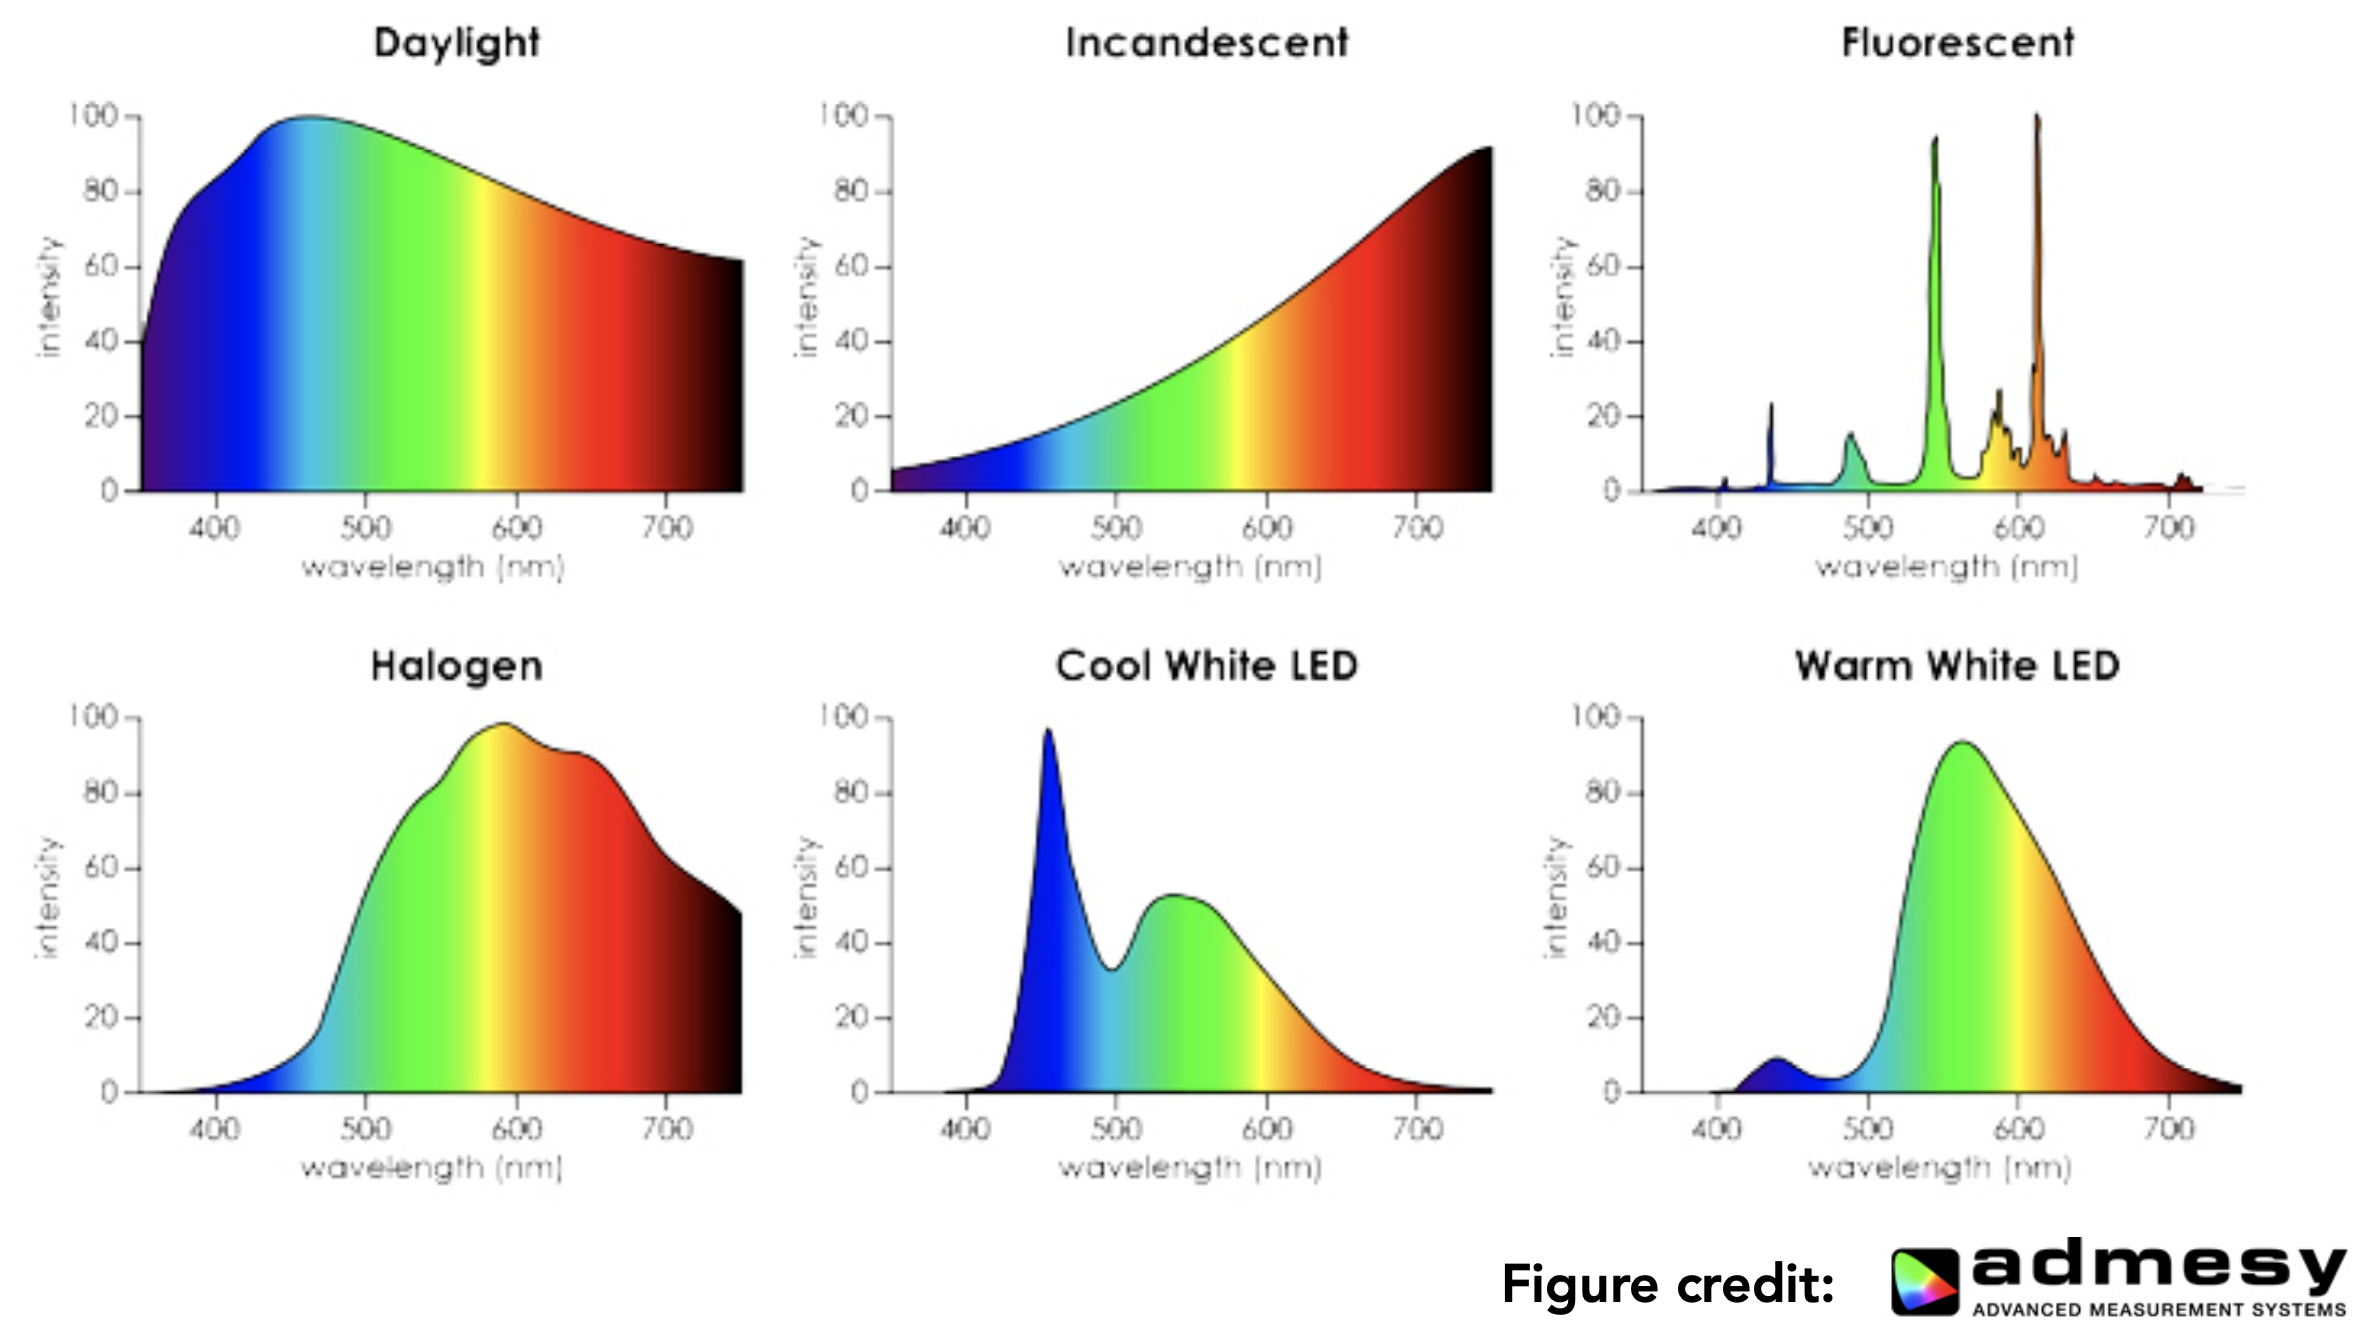
\includegraphics[scale=.2]{psd.png}
	\caption{常见光线的功率谱密度}
	\label{fig:psd}
\end{figure}

同时, 功率谱密度也满足可加性. 

而颜色, 应该是人对于不同光线的感知, 而不是不同光的波长. 我们接下来将讲解颜色的基础知识. 

\section{颜色生物学基础}

人的眼睛通过视网膜感受光线, 在视网膜上存在着两种细胞: 
\begin{itemize}
	\item 杆细胞 (Rods) 感受光线的明暗 (也就是灰度值) ; 
	\item 锥细胞 (Cones) 感受颜色. 锥细胞分为三种类型, 对不同的波长的光线的响应不同. 
\end{itemize}

\begin{figure}[H]
	\centering
	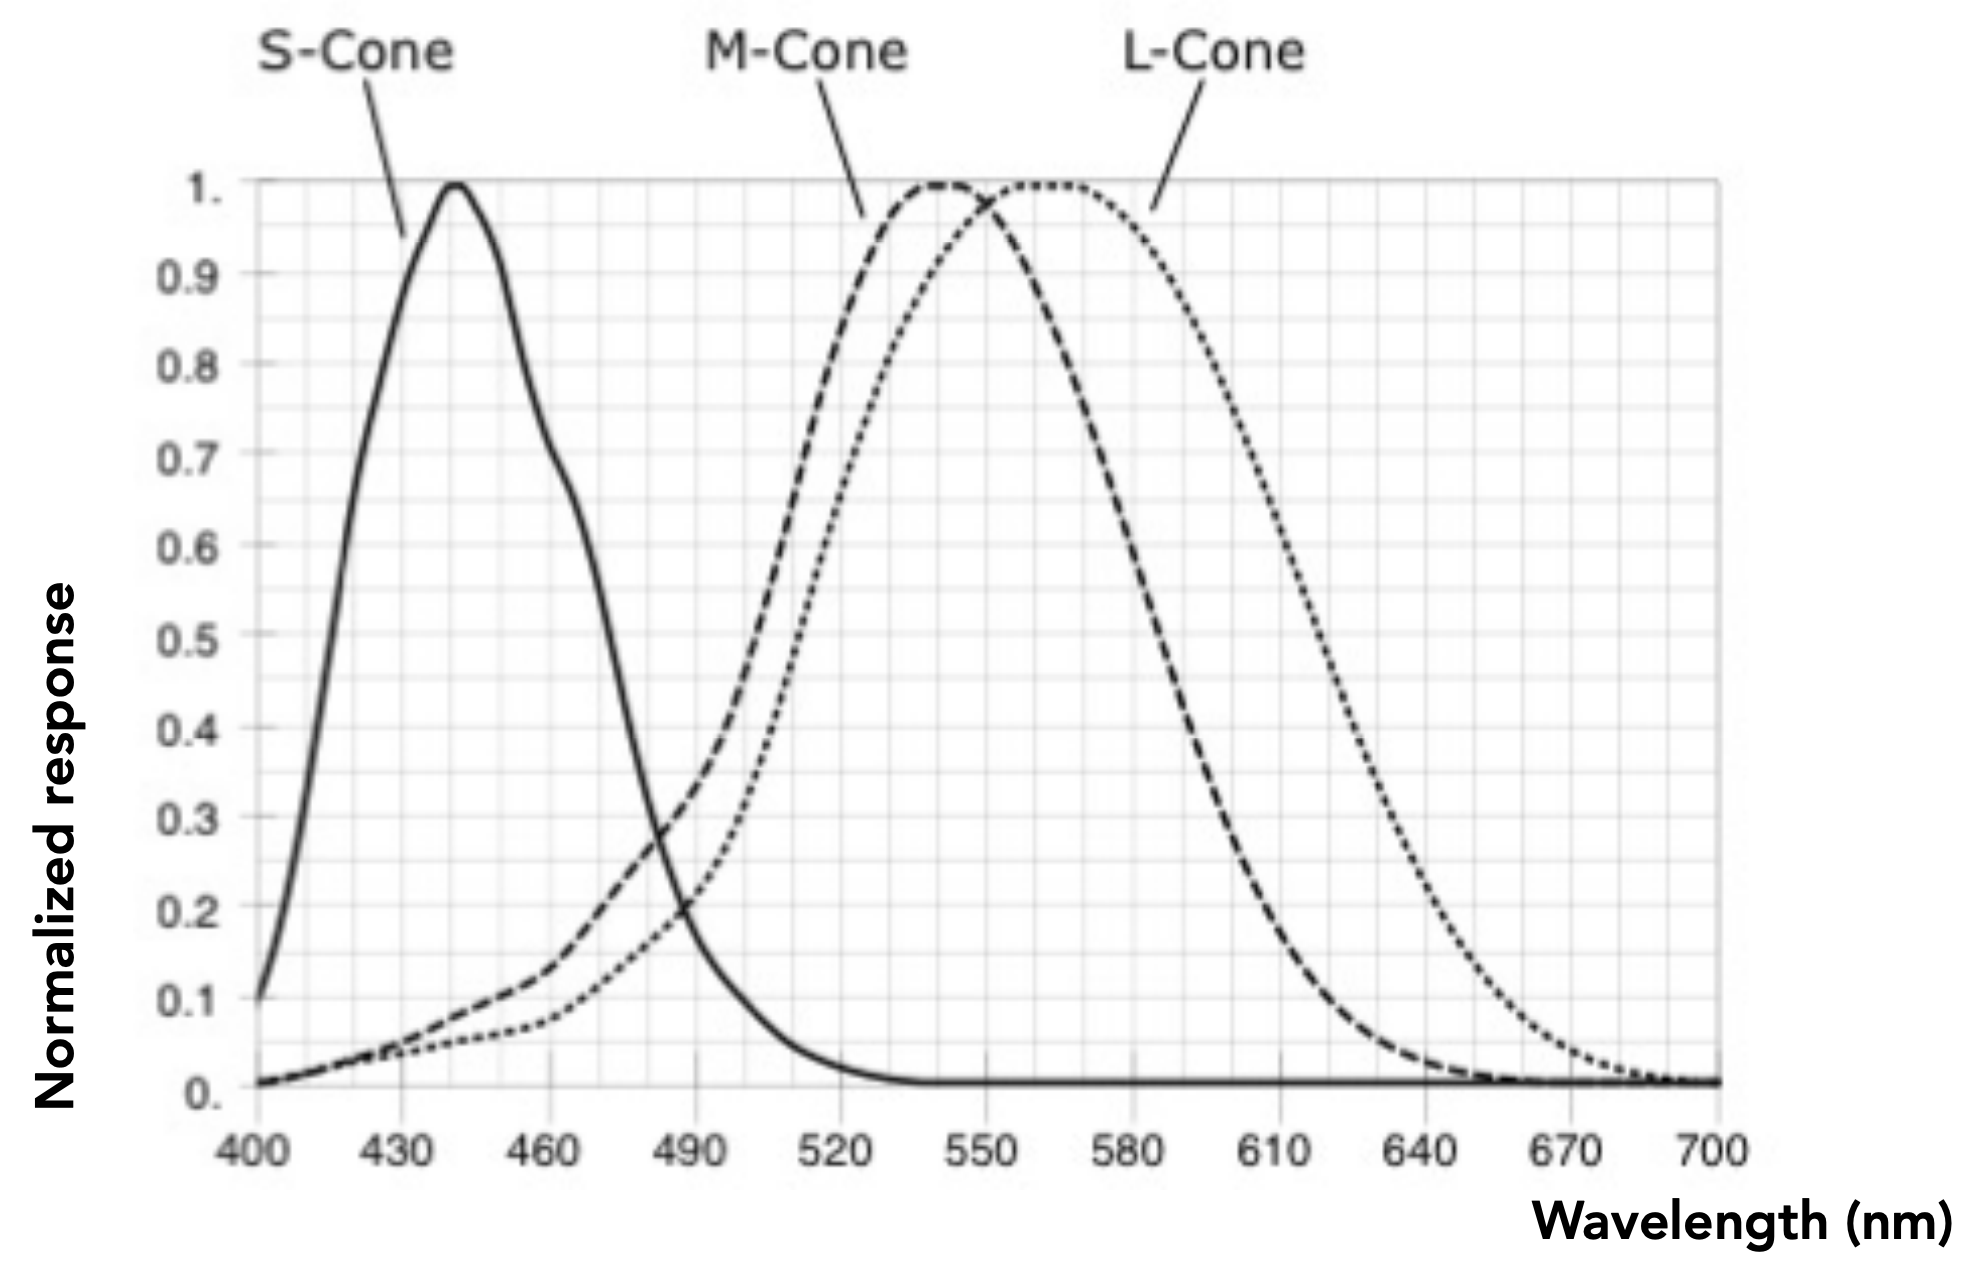
\includegraphics[scale=.2]{Cone.png}
	\caption{不同锥细胞对不同波长光线的响应}
	\label{fig:Cone}
\end{figure}

锥细胞可以分为S, M以及L三种, 分别对短波, 中波以及长波有更强的响应. 对于这三条谱功率密度曲线, 我们记为$r_S(\lambda),r_M(\lambda),r_L(\lambda)$, 那么对应的细胞感受到的能量是: 
\begin{equation}
	\begin{split}
		S &=\int r_{S}(\lambda) s(\lambda) d \lambda \\
		M &=\int r_{M}(\lambda) s(\lambda) d \lambda \\
		L &=\int r_{L}(\lambda) s(\lambda) d \lambda
	\end{split}
\end{equation}

对于人眼来说, 我们并不关注每一种波长的分布, 我们只关心三个响应量$(S,M,L)$. 因此, 即使是不同的光谱, 也有可能有相同的响应, 这就是同色异谱现象. 

\section{同色异谱}

\textbf{同色异谱 (Metamerism) }指的是两种不同的谱密度分布得到了相同响应量, 也就是相同的颜色. 因此, 当我们使用一些设备 (例如屏幕) 模拟其他颜色的时候, 并不需要按照原来的谱密度进行模拟. 

\section{颜色匹配}

\subsection{加色系统}

常见的加色系统为RGB系统, 在加色系统中, 越多的颜色混合, 得到的颜色越白. 在RGB系统中我们只需要得到RGB的谱密度$s_R(\lambda), s_G(\lambda), s_B(\lambda)$就可以通过$R s_{R}(\lambda)+G s_{G}(\lambda)+B s_{B}(\lambda)$得到对应的颜色. 

每一种波长的颜色通过人眼的方式进行匹配, 当两种颜色看上去一致的时候, 对应的RGB能量就是对应的结果. 但是可能存在某些颜色, 使用RGB不可以调整出来, 这个时候通过在原来的颜色上加入某些颜色使得颜色看上去一致. 这个时候对应的颜色分量能量我们视为负数. 

\subsubsection{CIE RGB 匹配方程}

CIE使用红色 (波长700nm) , 绿色 (波长546.1nm) 以及蓝色 (波长435.8nm) 三种颜色的光进行实验. 最终得到如下的结果

\begin{figure}[H]
	\centering
	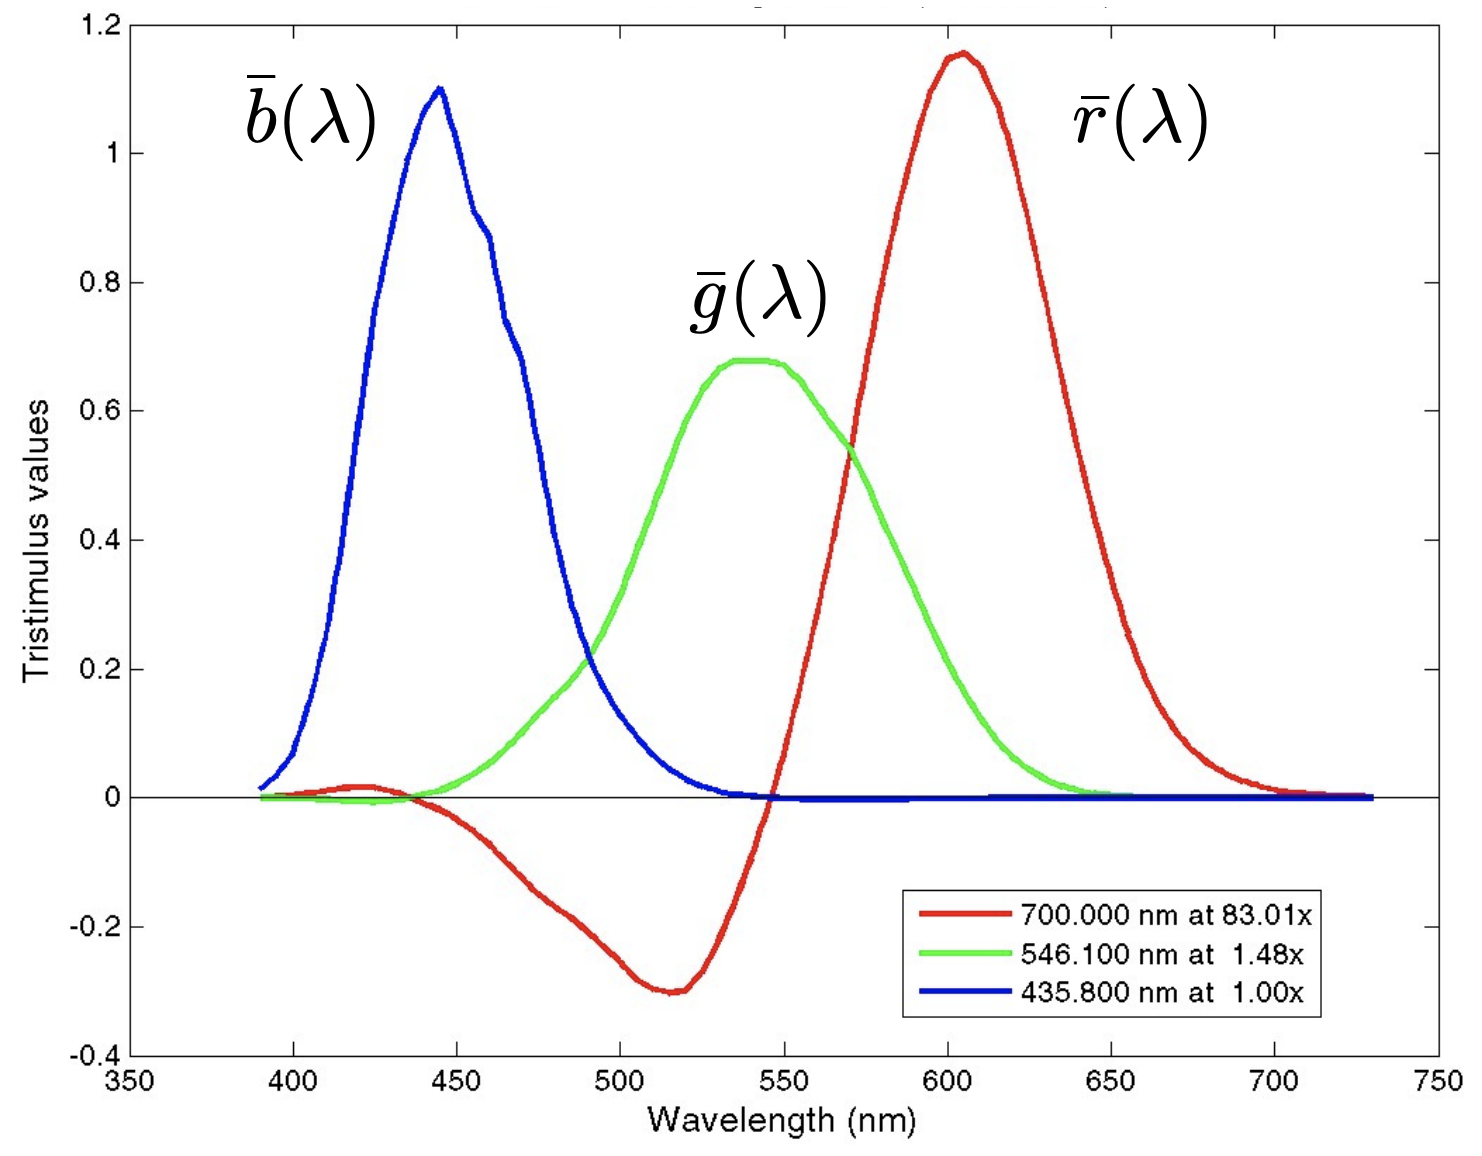
\includegraphics[scale=.2]{rgb.png}
	\caption{CIE使用RGB混合光线的结果}
	\label{fig:rgb}
\end{figure}

对应颜色的计算方式为: 

\begin{equation}
	\begin{split}
		R_{\mathrm{CIE} \text { RGB }} &=\int_{\lambda} s(\lambda) \bar{r}(\lambda) d \lambda \\
		G_{\mathrm{CIE} \text { RGB }} &=\int_{\lambda} s(\lambda) \bar{g}(\lambda) d \lambda \\
		B_{\mathrm{CIE} \text { RGB }} &=\int_{\lambda} s(\lambda) \bar{b}(\lambda) d \lambda
	\end{split}
\end{equation}

目前还会广泛使用sRGB (standardized RGB) 色彩空间, 通过一个标准的屏幕来调整其他的屏幕色彩. 这种方式被广泛使用, 但是其色域比较窄. 

\subsubsection{CIE XYZ 色彩空间}

XYZ色彩匹配函数是人造的函数. 其中Y的结果可以大致反应图片的亮度. 这样的设计不仅所有颜色能量都是正值, 同时可以表示出所有的颜色. 

\begin{figure}[H]
	\centering
	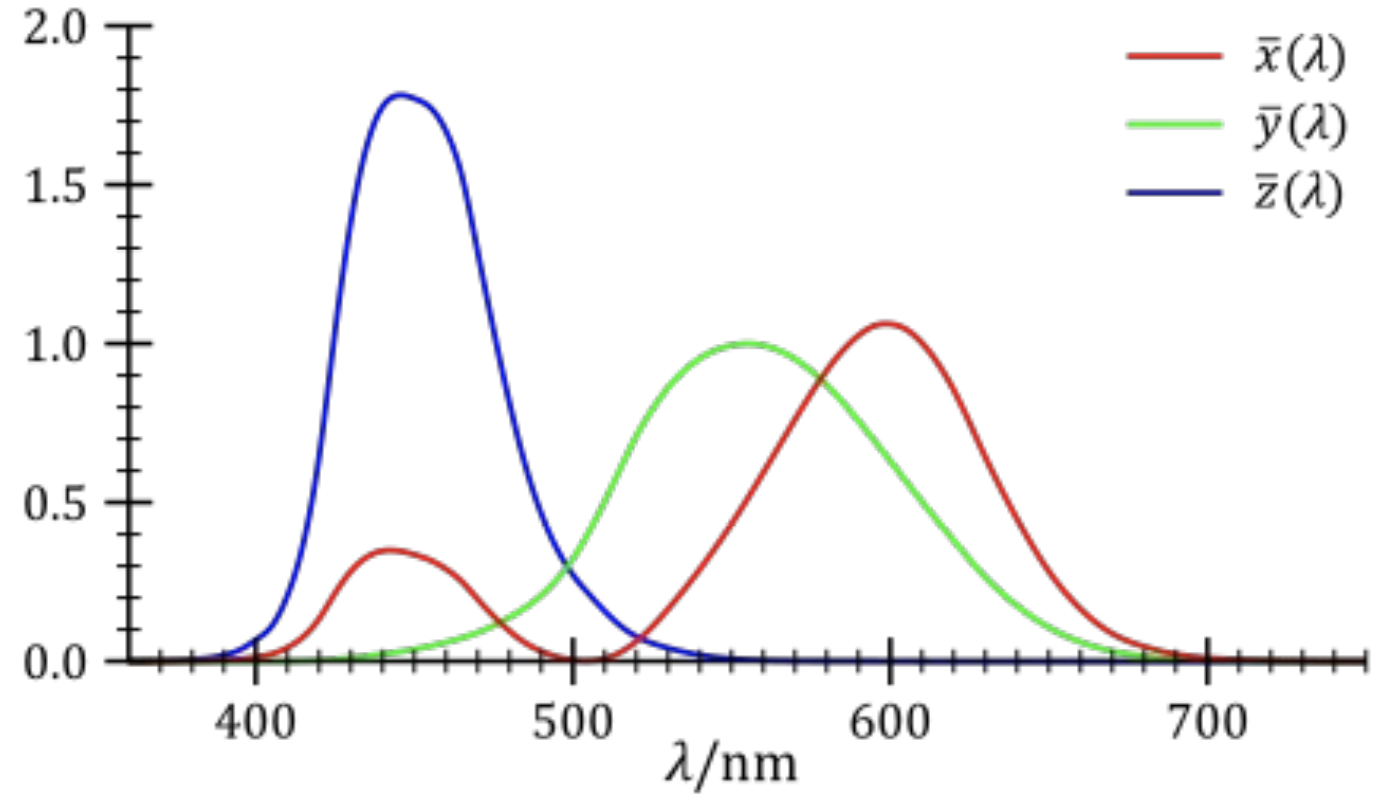
\includegraphics[scale=.2]{xyz.png}
	\caption{CIE XYZ匹配方程}
	\label{fig:xyz}
\end{figure}

我们令$x+y+z=1$, 通过归一化的方式, 我们可以将XYZ三维空间变成一个二维的空间进行表示: 
\begin{equation}
	\begin{split}
		x &=\frac{X}{X+Y+Z} \\
		y &=\frac{Y}{X+Y+Z} \\
		z &=\frac{Z}{X+Y+Z}
	\end{split}
\end{equation}

\begin{figure}[H]
	\centering
	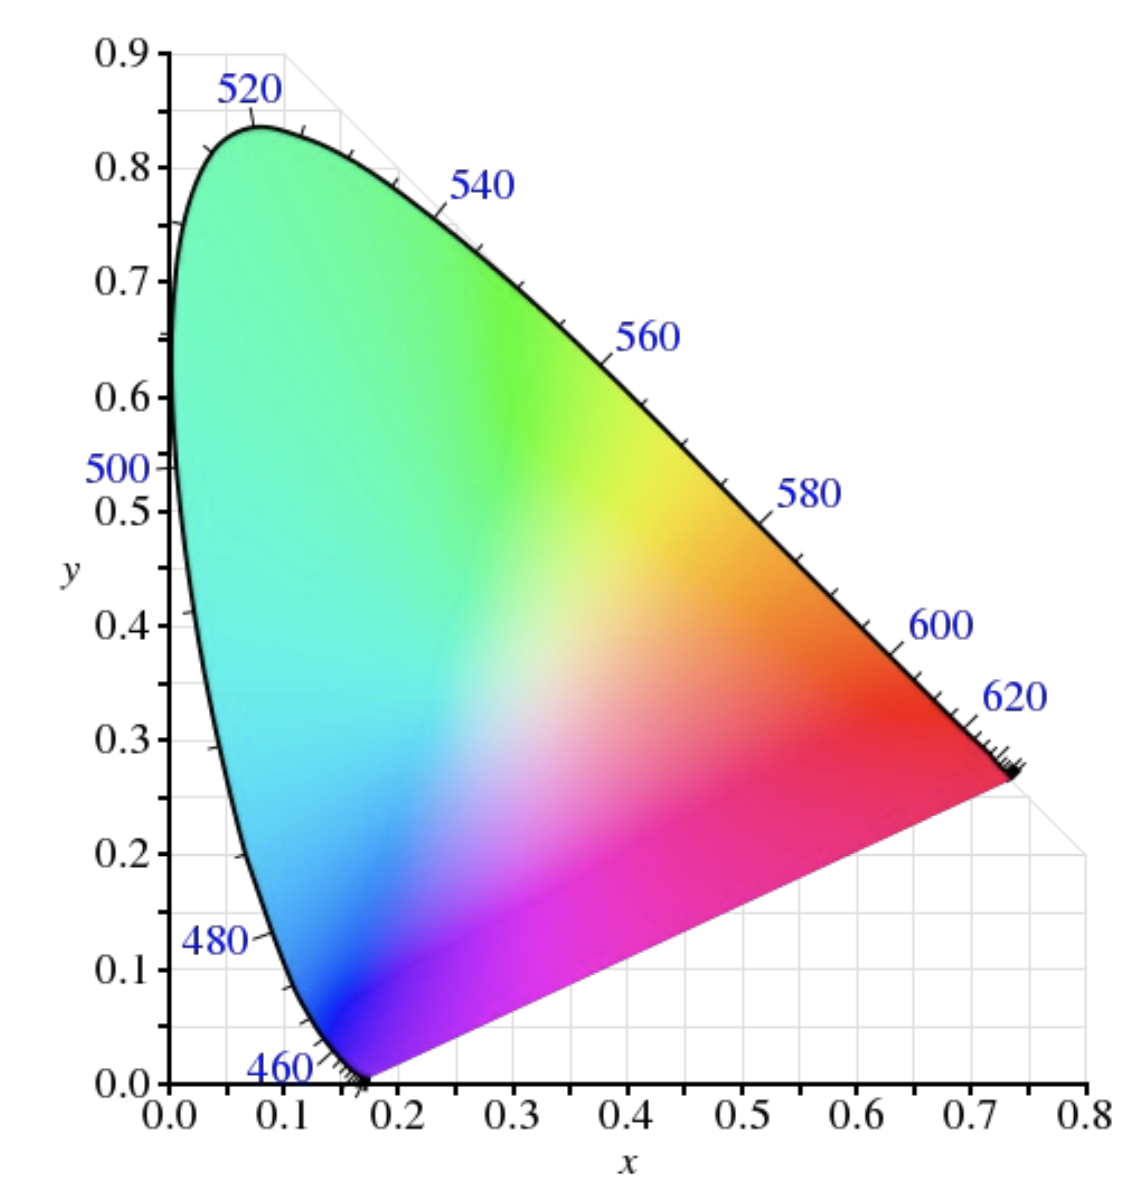
\includegraphics[scale=.2]{xyz2.png}
	\caption{CIE XYZ的颜色分布}
	\label{fig:xyz2}
\end{figure}

对于XYZ颜色的分布, 我们可以得到以下结果: 
\begin{itemize}
	\item 分布图的边缘都是纯色; 
	\item 中间的颜色没有那么纯; 
	\item 白色是最不纯的颜色, 位置在$(\frac{1}{3},\frac{1}{3})$处. 
\end{itemize}

\textbf{色域}指的是一系列颜色集所能得到的颜色的集合. 不同的颜色空间能够得到不同的色域. 

\subsection{感知颜色系统}

\subsubsection{HSV色彩空间}

\textbf{HSV色彩空间}包好色调 (Hue) , 饱和度 (Saturation) 以及亮度 (Lightness) 三个部分组成. 其中: 
\begin{itemize}
	\item 色调表示颜色的种类; 
	\item 饱和度表示颜色的纯度 (饱和度越低, 颜色越白) ; 
	\item 亮度表示颜色的亮度 (亮度越低, 颜色越黑) ; 
\end{itemize}

\begin{figure}[H]
	\centering
	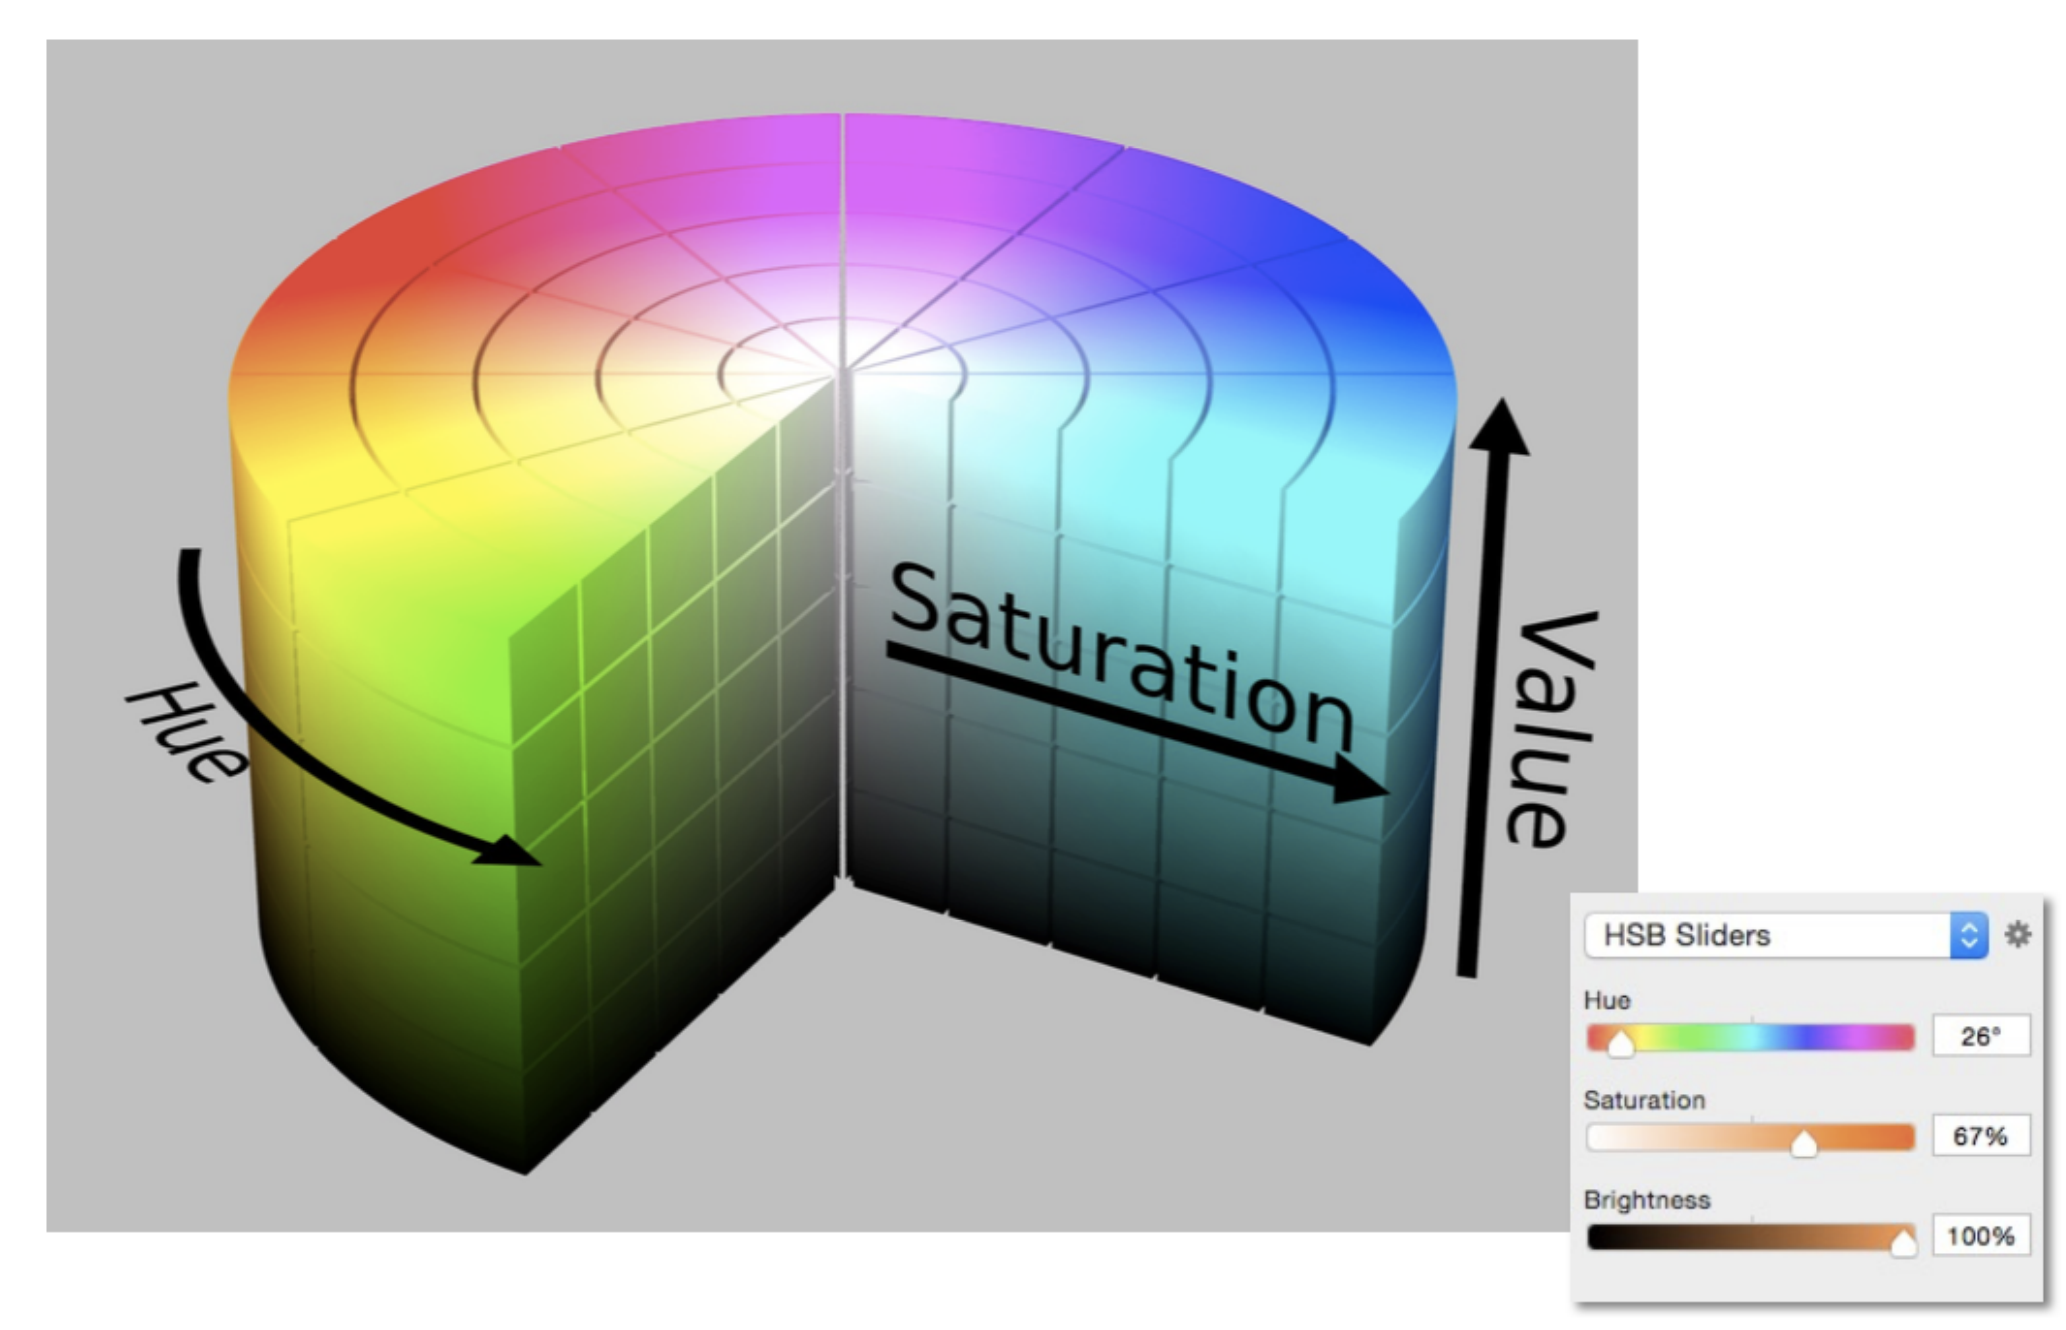
\includegraphics[scale=.2]{hsv.png}
	\caption{HSV颜色空间}
	\label{fig:hsv}
\end{figure}
正是这样, HSV颜色空间很适合用在颜色选择器上. 

\subsubsection{CIELAB空间 (L*a*b*) }

Lab颜色空间也是根据人的感知建立的颜色空间. 共包含了3个方向, L*方向指的是亮度, a*方向指的是红绿互补色对, b*方向是蓝黄互补色对. 之所以会选择这样的互补色对是因为黑白色, 红绿色以及黄蓝色是三对互补色. 

\begin{figure}[H]
	\centering
	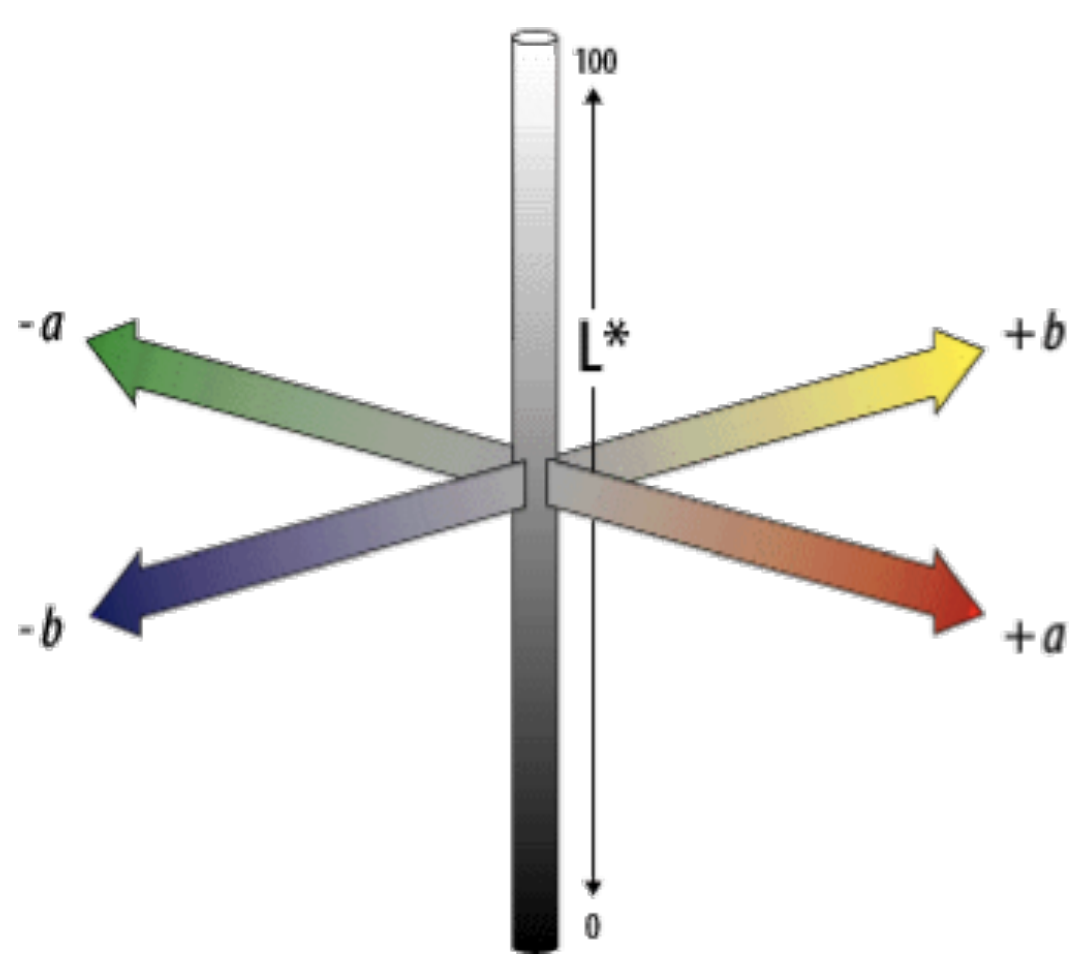
\includegraphics[scale=.2]{lab.png}
	\caption{L*a*b*颜色空间}
	\label{fig:lab}
\end{figure}

\subsection{减色系统}

\subsubsection{CMYK颜色空间}

CMYK颜色空间是一种减色系统, 当混合的颜色越多, 得到的颜色越黑. CMYK广泛应用于打印中. CMYK包含4种基础色, 分别是青色 (Cyan) , 品红 (Magenta) , 黄色 (Yellow) 和黑色 (Key) . 使用前三种颜色就可以得到黑色, 但是基于成本原因, 还是加入了K降低成本. 

\begin{figure}[H]
	\centering
	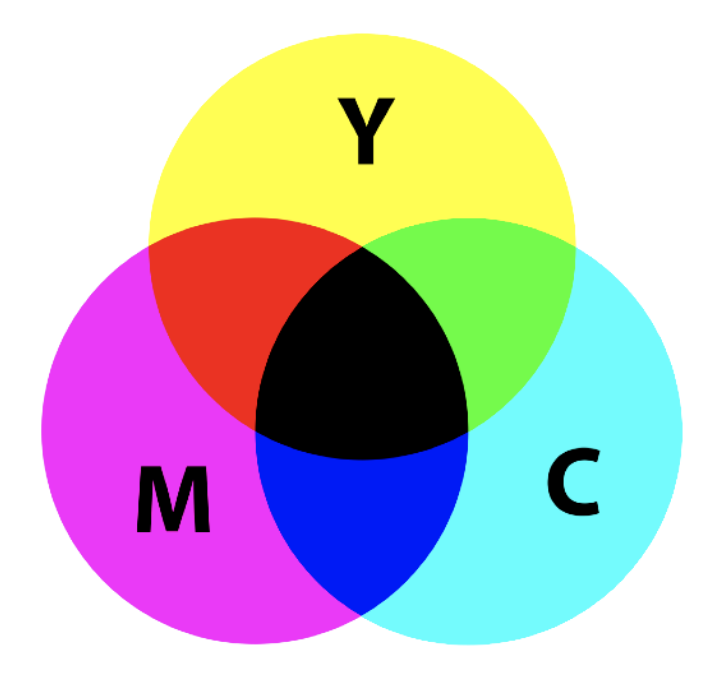
\includegraphics[scale=.2]{cmyk.png}
	\caption{CMYK颜色空间}
	\label{fig:cmyk}
\end{figure}

\chapter{动画}

\textbf{动画 (Animation) }是一门``让物体变活”的技术. 可以理解为模型在不同的时间具有不同的几何形状. 根据人眼的视觉暂留效应, 动画只需要在一定时间内连续播放多张图片就有物体在连续运动的效果. 例如对于视觉暂留只需要24fps就可以达到动画效果, 视频的帧率为24fps, 而虚拟现实需要达到90fps才不会产生眩晕感. 

\section{关键帧动画}

\textbf{关键帧动画 (Keyframe Animation) }包含两个部分, 一部分是关键帧 (Keyframe) , 是动画中比较重要的部分. 两个关键帧之间是过渡帧 (Tweens) . 关键帧动画的问题的重要问题就是插值问题. 

插值方法有很多, 例如线性插值, 样条插值等方法. 我们希望能有更加自然的插值方式, 因此会更多的使用样条插值的方法. 

\section{物理模拟}

物理模拟最简单应用就是牛顿定理: 
\begin{equation}
	F=ma
\end{equation}

所谓物理模拟就是通过模拟出不同的物理公式来仿真出不同的物理效果. 

\subsubsection{质点弹簧系统}

这里我们介绍最简单但是最实用的物理系统——\textbf{质点弹簧系统 (Mass Spring System) }. 

质点弹簧系统中最基本的单元是一根弹簧以及左右连接的两个质点. 

\begin{figure}[H]
	\centering
	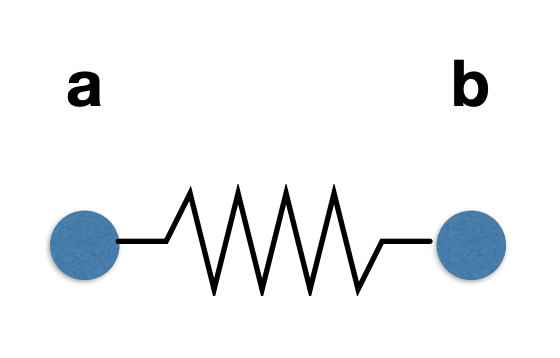
\includegraphics[scale=.3]{zhidiantanhuang.png}
	\caption{质点弹簧系统的基本单元}
	\label{fig:zdth}
\end{figure}

假设弹簧没有长度, 根据胡克定律可以得到: 
\begin{equation}
	\mathbf{f}_{a \rightarrow b}=k_{S}(\mathbf{b}-\mathbf{a})
\end{equation}

弹簧被拉的越长, 受到的力越大. 同时, 我们又知道力的作用是相互的, 所以有: 
\begin{equation}
	\mathbf{f}_{b \rightarrow a}=-\mathbf{f}_{a \rightarrow b}
\end{equation}

这里假设弹簧是没有长度的, 但实际上弹簧在不受力时也有一定的长度, 因此胡克定律应该改写为: 
\begin{equation}
	\mathbf{f}_{a \rightarrow b}=k_{s} \frac{\mathbf{b}-\mathbf{a}}{\|\mathbf{b}-\mathbf{a}\|}(\|\mathbf{b}-\mathbf{a}\|-l)
\end{equation}

其中, $l$是弹簧的原长 (Rest Length) . 为了能够更好的说明, 我们引入以下记号来表示位置, 速度和加速度: 
\begin{equation}
	\begin{split}
	&	x \\
	&	\dot{x}=v \\
	&	\ddot{x}=a
	\end{split}
\end{equation}

\subsection{能量损耗}

任何一个弹簧在拉长之后都会发生震动, 为了使弹簧不发生震动, 我们需要引入一个外部摩擦力 (Damping Force) , 保证质点可以停下来. 对于任何一个物体我们希望它停下, 就需要一个和物体相反的力. 这个力可以表示为: 
\begin{equation}
	\mathbf{f}=-k_d\mathbf{\dot{b}}
\end{equation}

这样的描述带来的问题是会让所有的质点运动停下. 如果出现一个弹簧的两个端点同时进行匀速直线运动, 这个时候外部摩擦力就会让整个运动停下, 但是实际上弹簧并没有发生震动, 因此我们需要引入内部摩擦力: 

\begin{equation}
	\mathbf{f}_{\mathbf{b}}=-k_{d}\frac{\mathbf{b}-\mathbf{a}}{\|\mathbf{b}-\mathbf{a}\|}(\dot{\mathbf{b}}-\dot{\mathbf{a}})\cdot \frac{\mathbf{b}-\mathbf{a}}{\|\mathbf{b}-\mathbf{a}\|}
\end{equation}

在这个式子中, 我们考虑两个质点间的相对速度 (这样可以避免相对运动的问题) . 同时, 只有在两个质点连线方向上的速度投影才可以引起弹簧长度改变. 例如$a$不动, $b$相对于$a$做圆周运动, 这个时候并没有使弹簧长度发生改变, 这个速度不引起弹簧内部的能量损耗. 

\subsubsection{形状表示}

通过这些弹簧进行连接, 我们可以得到各种材料. 这里, 我们使用质点弹簧系统对布料进行模拟. 

\begin{figure}[H]
	\centering
	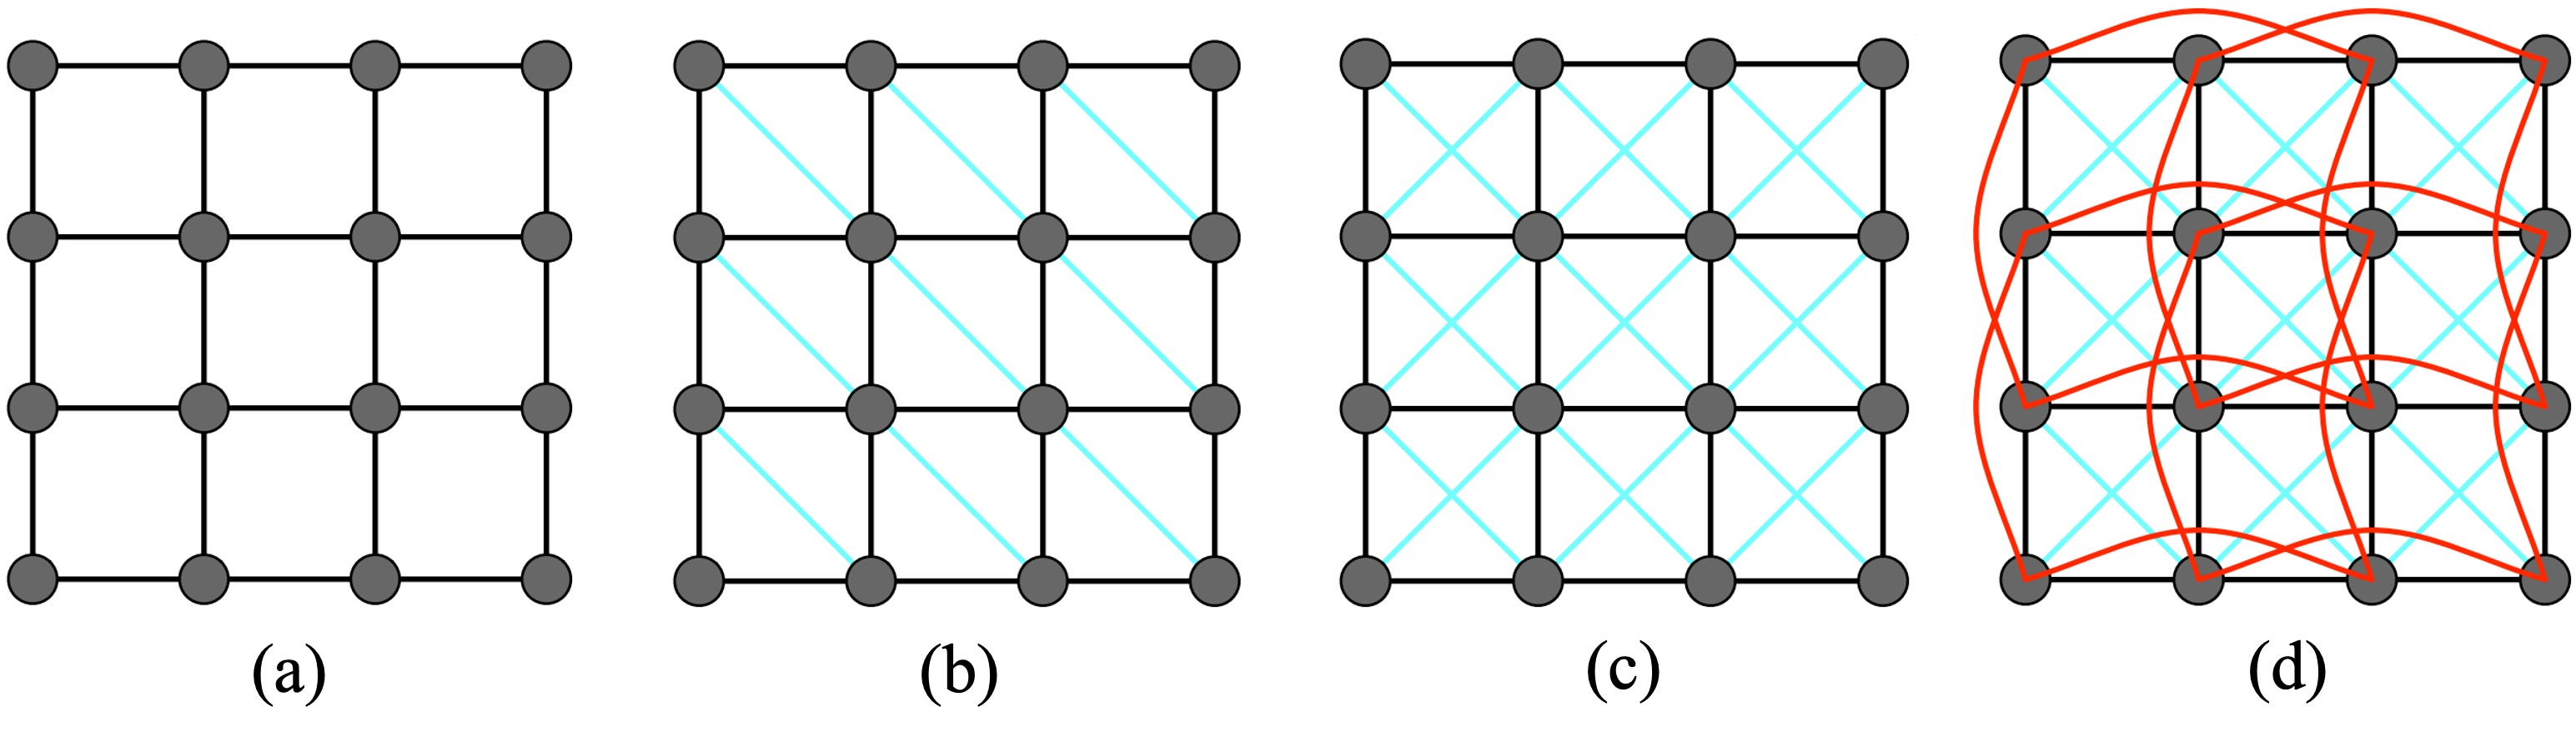
\includegraphics[scale=.1]{buliao.jpg}
	\caption{质点弹簧系统模拟布料}
	\label{fig:buliao}
\end{figure}

对于图\ref{fig:buliao}(a), 不能很好的抵抗切变, 同时布料很难被折叠, 但是这个结构可以进行折叠 (Out-of-plane Bending) . 因此这样的设计是不合理的. 在图\ref{fig:buliao}(b)中加入斜的对角线来抵抗切变, 但是依然不能解决折叠的问题, 并且整个布是各向异性的. 在图\ref{fig:buliao}(c)中再加入一条对角线, 这样就可以抵抗对角线上折叠的力, 并且整个布料是各向同性的. 但是在水平和垂直方向依然可以折叠. 在图\ref{fig:buliao}(d)中, 都在间隔一个点两个点之间加入一条线, 这样就可以抵抗水平和垂直的折叠. 在这里, 蓝线是比较强的抵抗, 但是红线的抵抗比较弱. 


\section{粒子系统}

现实生活中很多物体都是由大量的粒子组成的. 我们称之为\textbf{粒子系统}. 对于粒子系统, 可能需要大量的粒子来模拟复杂的现象, 并且需要一些加速结构加快粒子作用力的计算. 粒子系统的计算分为以下几个步骤: 
\begin{enumerate}
	\item 产生新的粒子 (如果有需要) ; 
	\item 计算每一个粒子受到的作用力; 
	\item 更新每一个粒子的位置和速度; 
	\item 移除死亡的粒子 (如果有需要) ; 
	\item 渲染粒子. 
\end{enumerate}


在粒子系统中可以考虑许多力作用, 引力和斥力包括万有引力, 电磁力, 弹力, 推进力. 阻尼力包括摩擦力, 空气阻力, 以及黏力. 同时还要考虑碰撞产生的力. 

\section{动力学}

动力学包括\textbf{正向动力学 (Forward Kinematics) }以及\textbf{逆向动力学 (Inverse Kinematics) }. 如图\ref{fig:gg}所示是一个人体骨骼的抽象. 在正向动力学中, 我们会知道所有关节的旋转角度, 推断出尖端所在的位置. 在逆向动力学中, 已知尖端的位置, 需要推断出


\begin{figure}[H]
	\centering
	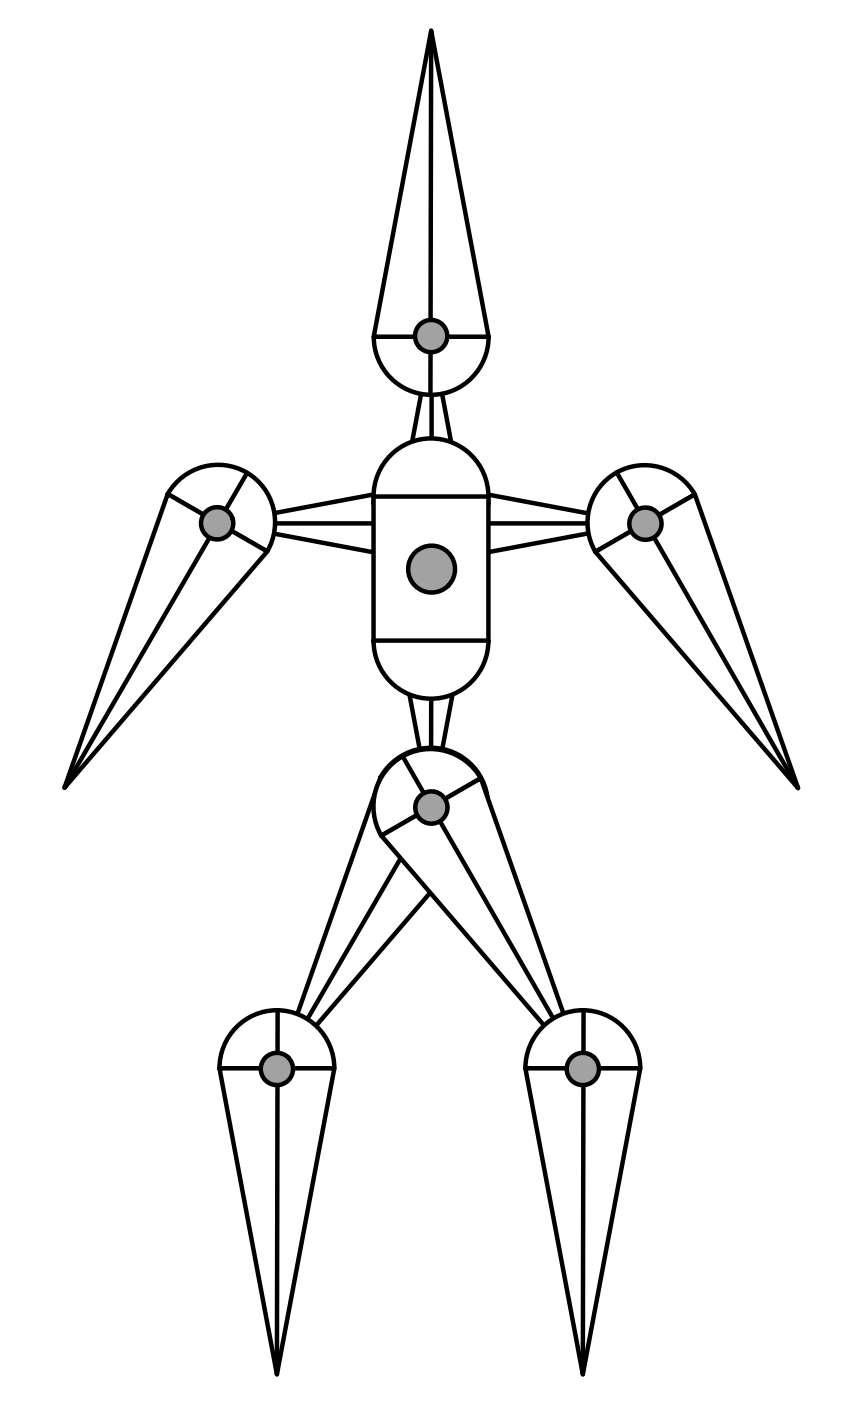
\includegraphics[scale=.3]{rig.png}
	\caption{人体骨骼的抽象}
	\label{fig:gg}
\end{figure}

\subsection{正向动力学}

在正向动力学中, 计算尖端位置主要通过三角函数进行计算. 以下图为例, 是一个简单的骨骼系统计算尖端位置的方法. 

\begin{figure}[H]
	\centering
	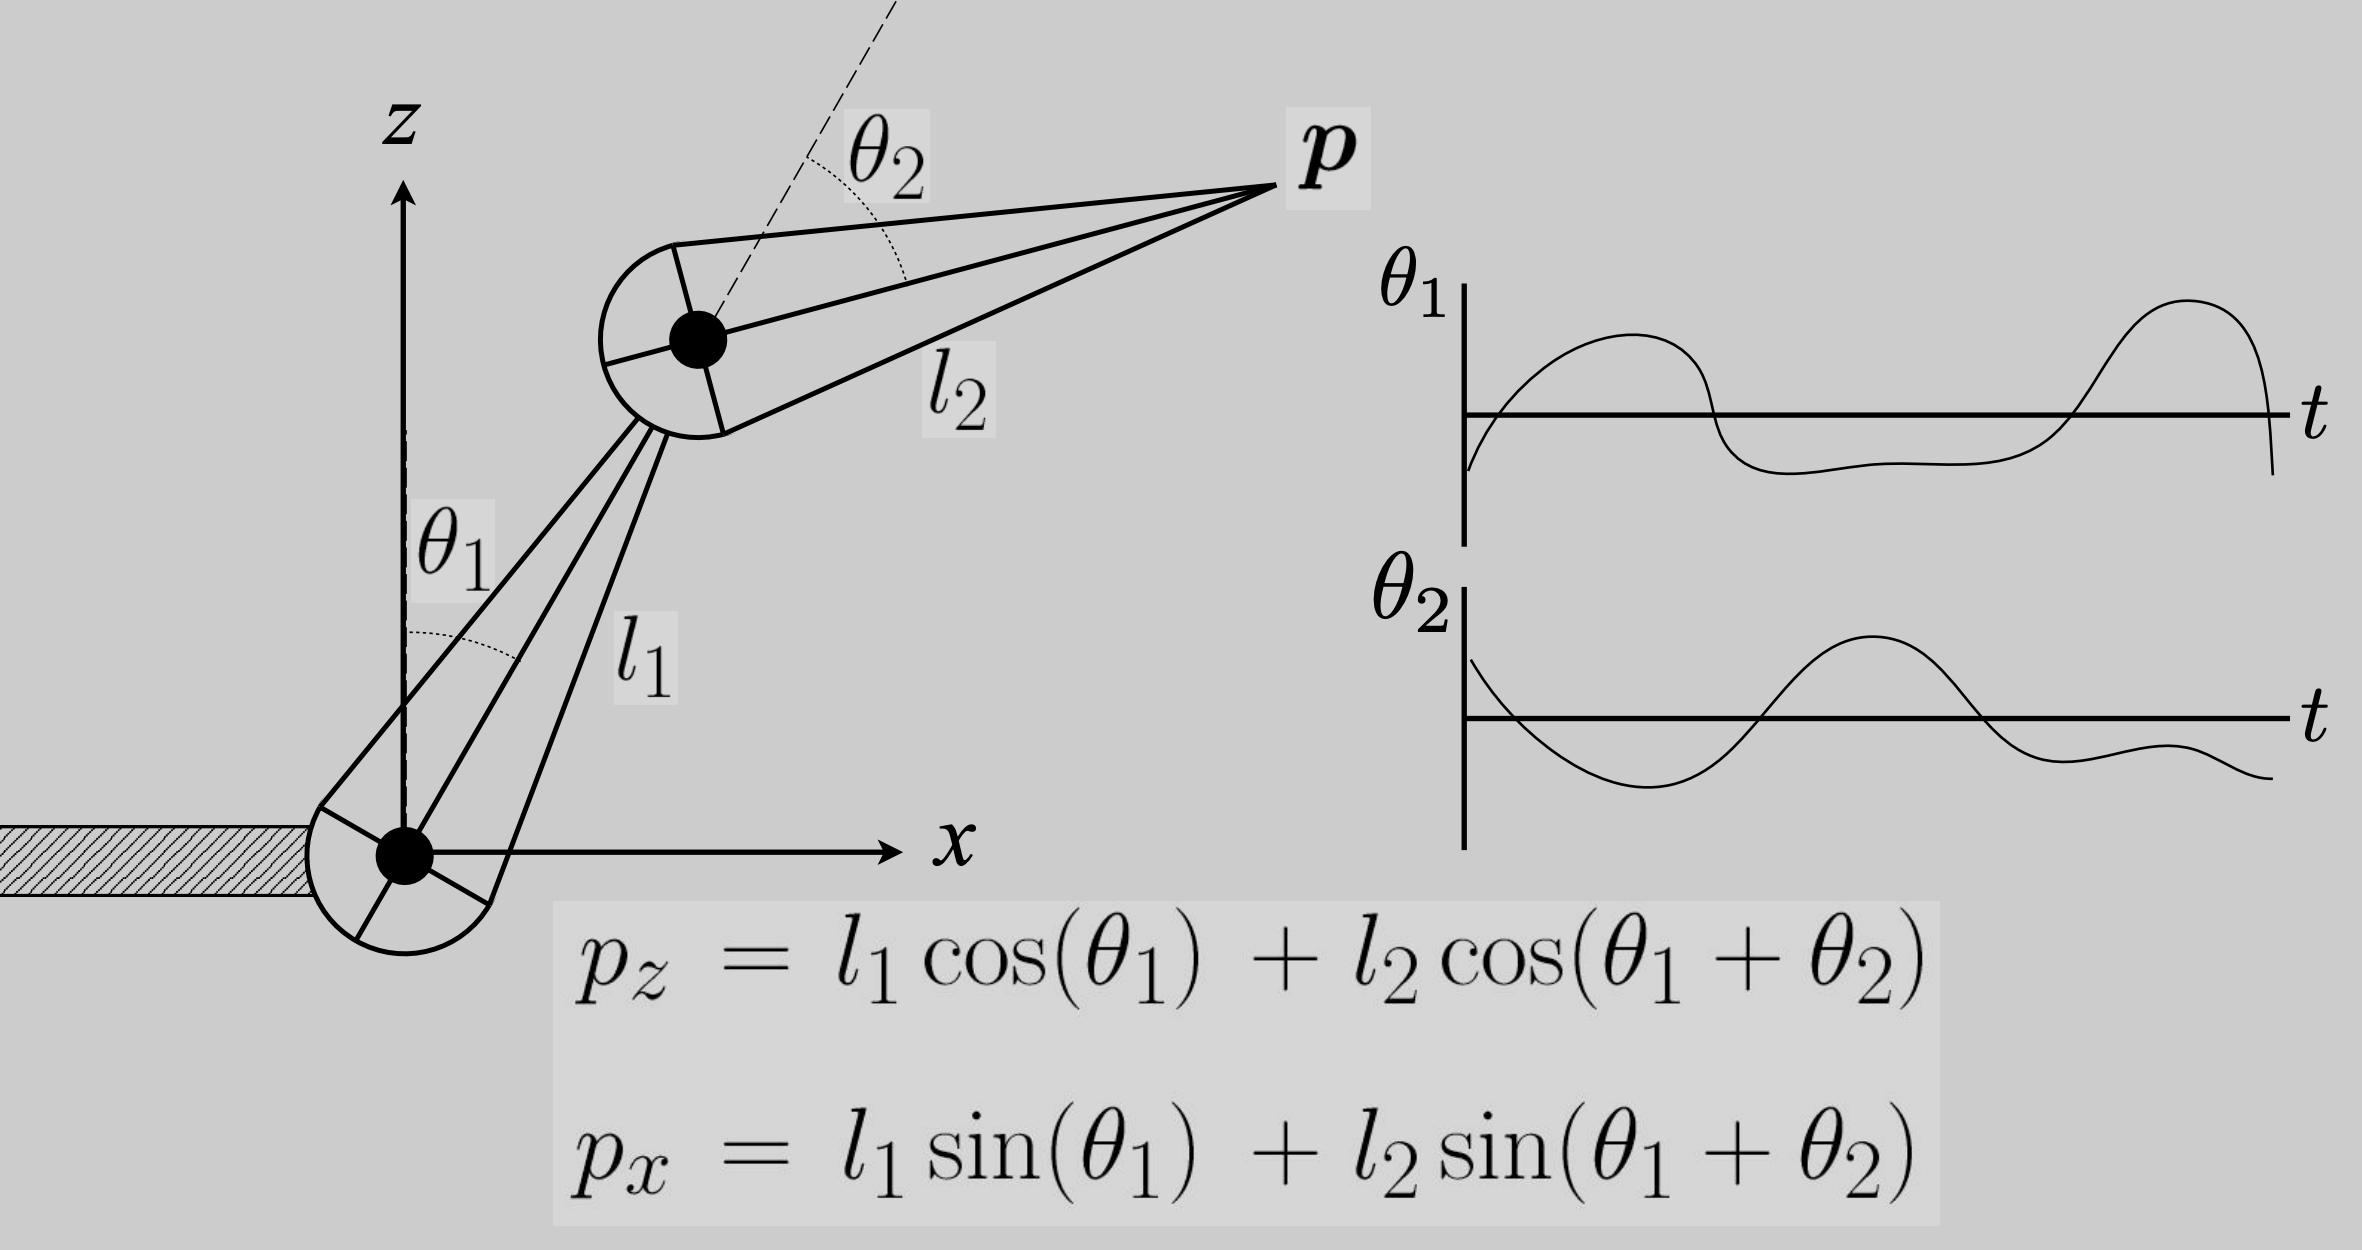
\includegraphics[scale=.2]{FK.png}
	\caption{正向运动学计算尖端位置}
	\label{fig:fk}
\end{figure}

正向动力学能够方便的控制骨骼方向, 并且计算方便; 但是得到的物理模拟不一定连续, 并且对于艺术家来说, 调整工作非常浪费时间. 

\subsection{方向动力学}

反向动力学中, 在得到尖端位置后我们需要计算各个关节的旋转角度. 下图提供了一个简单关节的计算方式. 

\begin{figure}[H]
	\centering
	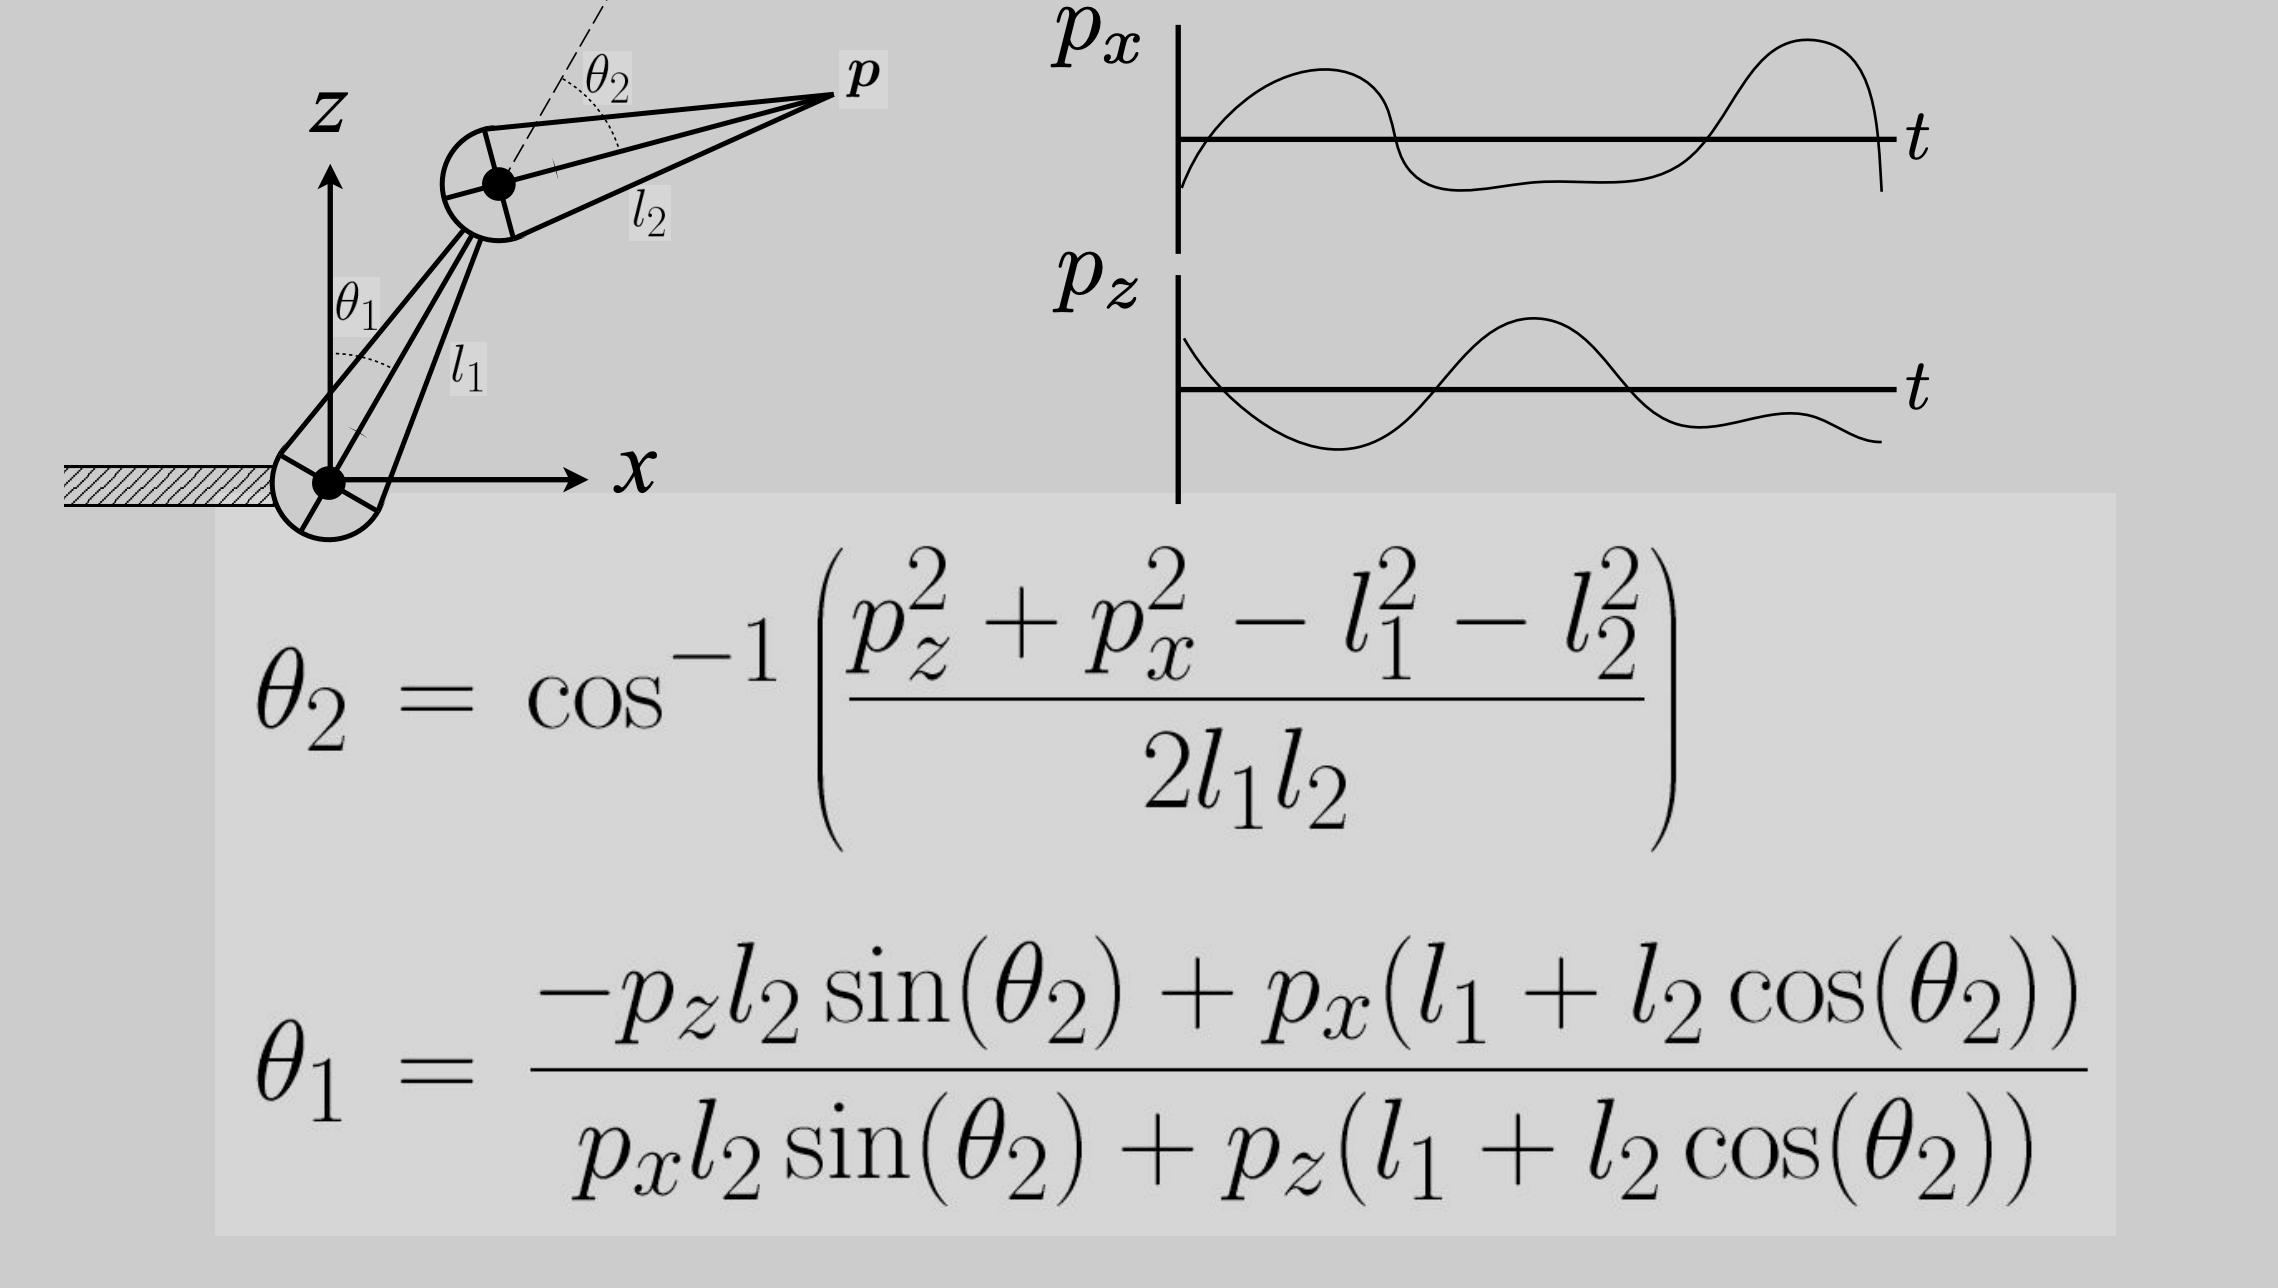
\includegraphics[scale=.2]{IK.png}
	\caption{反向运动学计算关节旋转角度}
	\label{fig:ik}
\end{figure}

在反向动力学中主要面对以下几个问题: 
\begin{enumerate}
	\item 解不一定唯一; 
	\item 关节连接越多, 计算越麻烦; 
	\item 在某些地方可能不存在解. 
\end{enumerate}

当然目前也存在很多方法解决这些问题, 例如对于N连接的IK问题: 

\begin{itemize}
	\item 选择初始设定; 
	\item 定义错误度量方式; 
	\item 将错误的梯度作为设定之一; 
	\item 使用梯度下降计算梯度. 
\end{itemize}

\section{单粒子模拟}

我们假设粒子在一个力场之中, 力场中的任何一个点都定义了这个点处粒子收到的力的大小和方向, 目的是在知道粒子的起点后, 我们需要计算出力在场中的运动轨迹. 

\begin{figure}[H]
	\centering
	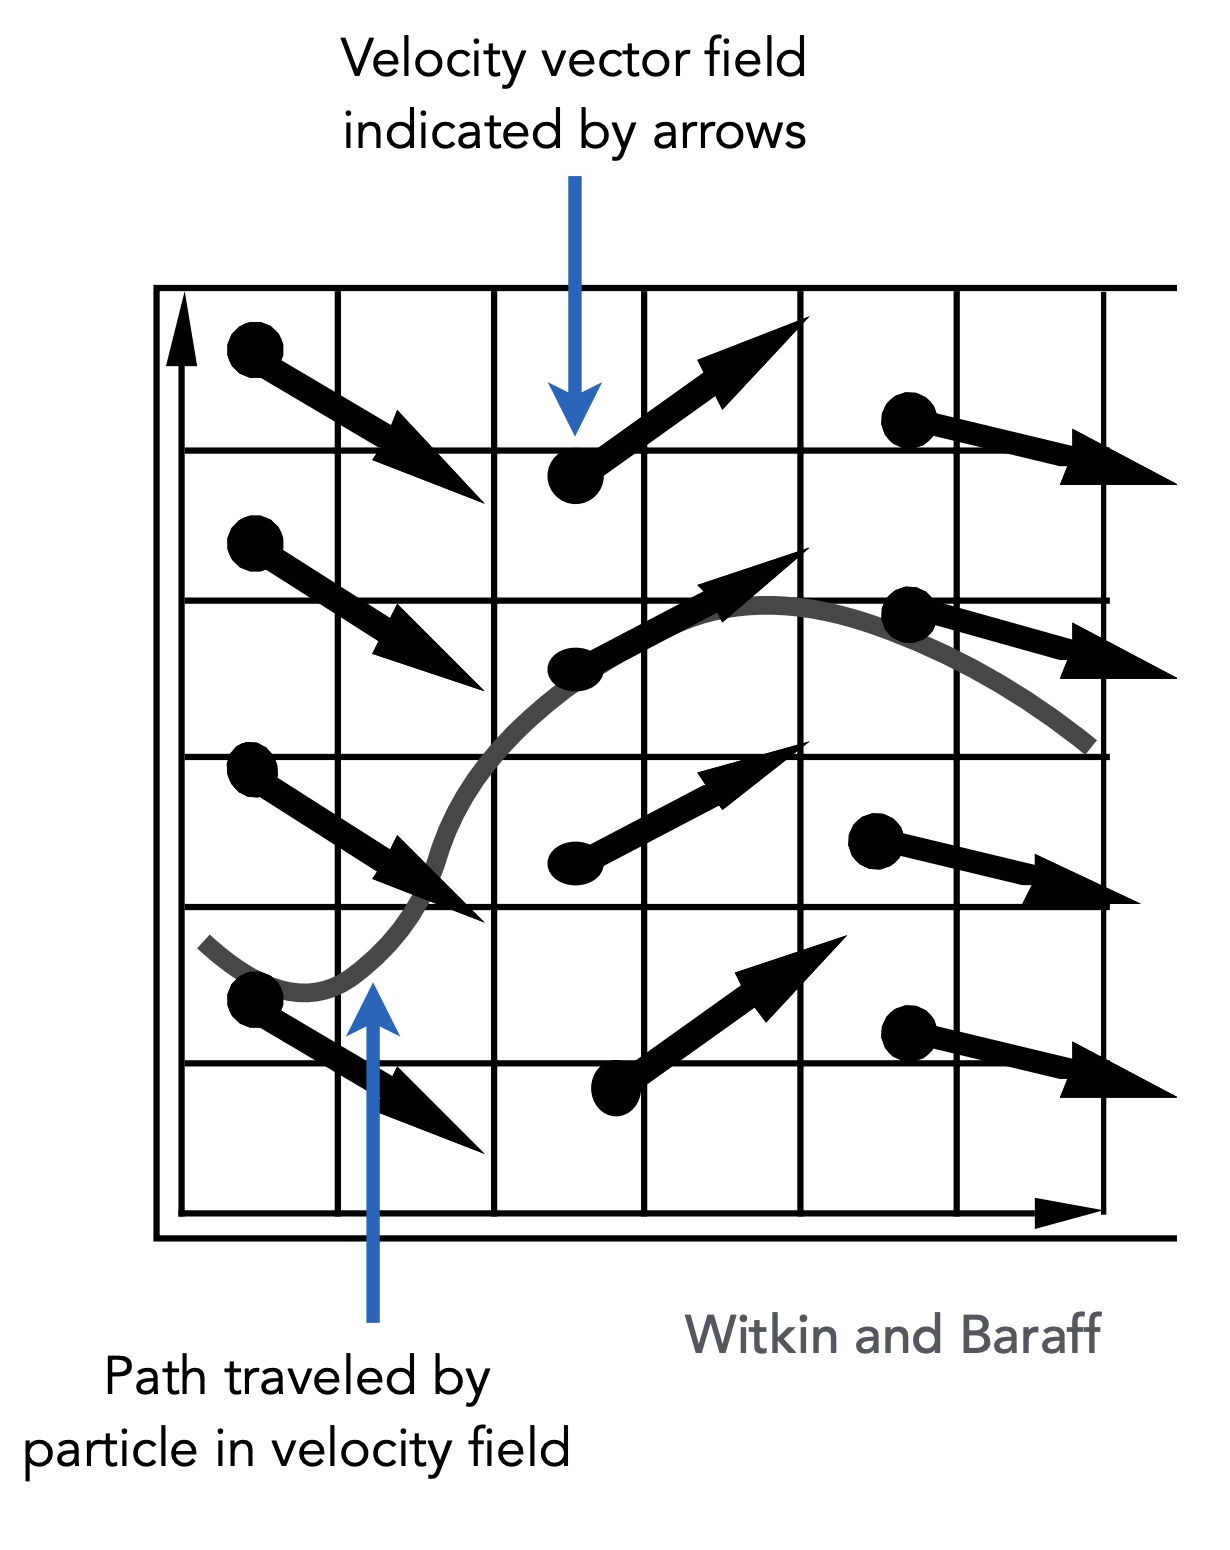
\includegraphics[scale=.2]{OED.png}
	\caption{力场}
	\label{fig:OED}
\end{figure}

在这样的系统中, 我们需要解的是$x$关于$t$的常微分方程, 也就是: 
\begin{equation}
	\frac{d x}{d t}=\dot{x}=v(x, t)
\end{equation}

\subsection{欧拉方法}

\textbf{欧拉方法 (Euler‘s Method) }非常的简单且常用, 但是往往不稳定, 方法可以表示为: 
\begin{equation}
	\begin{split}
		\mathbf{x}^{t+\Delta t} &=\mathbf{x}^{t}+\Delta t \dot{\mathbf{x}}^{t} \\
		\dot{\mathbf{x}}^{t+\Delta t} &=\dot{\mathbf{x}}^{t}+\Delta t \ddot{\mathbf{x}}^{t}
	\end{split}
\end{equation}

欧拉方法错误的多少和步长的选择有关, 步长越小, 模拟出的路径误差越小. 

\begin{figure}[H]
	\centering
	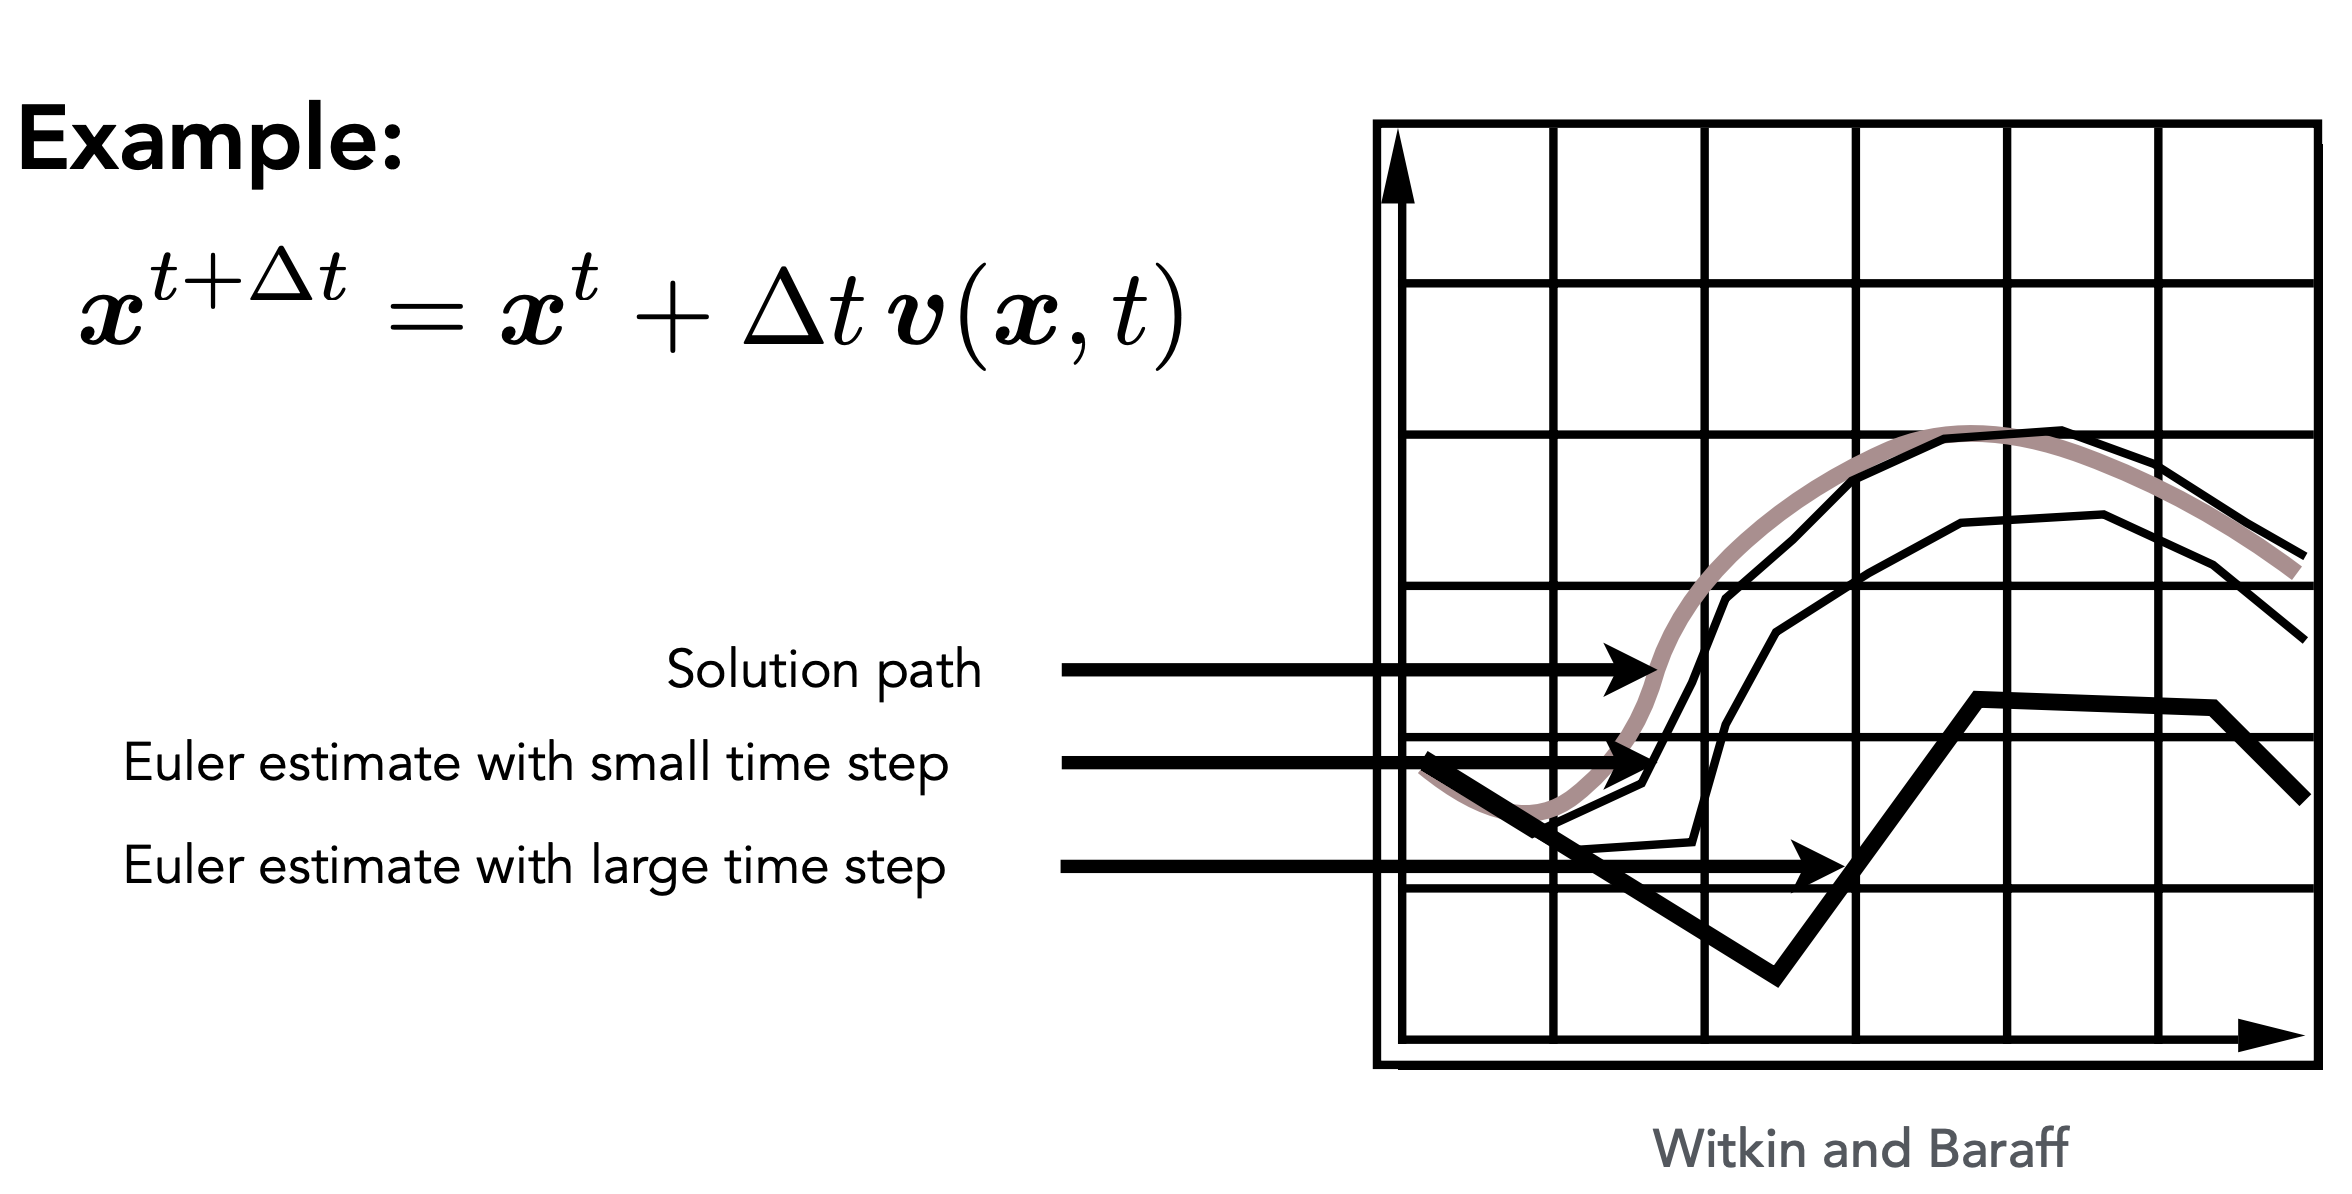
\includegraphics[scale=.2]{buchang.png}
	\caption{步长的选择对模拟路径的影响}
	\label{fig:buchang}
\end{figure}

另一方面, 即使是减少步长, 在某些力场中依然会有不稳定的情况产生. 例如在匀速圆周运动的力场中, 粒子可以做匀速圆周运动. 但是使用欧拉方法后, 模拟出的路径会一步一步远离力场中心. 这就被称作不稳定性. 

\begin{figure}[H]
	\centering
	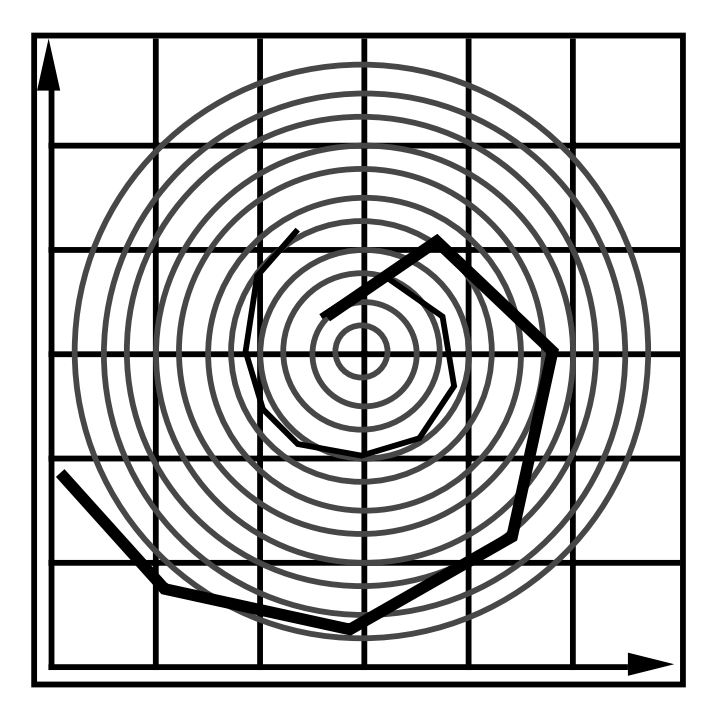
\includegraphics[scale=.2]{ysyzlichang.png}
	\caption{匀速圆周力场对模拟路径的影响}
	\label{fig:ysyz}
\end{figure}

错误和不稳定性是衡量路径模拟的指标. 错误会在每一步积累, 降低路径模拟的准确性. 而不稳定性也是影响路径模拟效果的因素之一. 目前也有一些方法来解决模拟中的不稳定性. 

\subsubsection{中点法}

中点法的步骤如下: 
\begin{enumerate}
	\item 使用欧拉方法计算下一步粒子的位置; 
	\item 计算中点下一步移动的梯度; 
	\item 使用中点的梯度更新该点的位置. 
\end{enumerate}

\begin{equation}
	\begin{split}
		x_{mid} &=x(t)+\Delta t / 2 \cdot v(x(t), t) \\
		x(t+\Delta t) &=x(t)+\Delta t \cdot v\left(x_{mid}, t\right)
	\end{split}
\end{equation}



\subsection{自适应步长}

自适应步长的方法可以通过误差分析计算所需要步长的大小, 具体的步骤如下: 

\begin{enumerate}
	\item 计算步长为$T$时欧拉方法移动的位置$x_T$; 
	\item 计算步长为$T/2$时欧拉方法移动的位置$x_{T/2}$; 
	\item 计算误差$||x_T-x_{T/2}||$; 
	\item 如果误差大于阈值, 减小步长并重复以上过程. 
\end{enumerate}

\subsection{隐式欧拉方法}

在隐式欧拉方法中, 我们需要计算出$\mathbf{x}^{t+\Delta t}$以及$\dot{\mathbf{x}}^{t+\Delta t} $的结果. 可以使用牛顿法求解, 但是求解相对不方便. 但是具有更好地稳定性. 

\begin{equation}
	\begin{split}
		\mathbf{x}^{t+\Delta t} &=\mathbf{x}^{t}+\Delta t \dot{\mathbf{x}}^{t+\Delta t} \\
		\dot{\mathbf{x}}^{t+\Delta t} &=\dot{\mathbf{x}}^{t}+\Delta t \ddot{\mathbf{x}}^{t+\Delta t}
	\end{split}
\end{equation}

这里我们可以对稳定性进行定义. 我们使用每一步的误差以及整体累计的误差表示方法的稳定性. 误差本身没有太多意义, 但是误差的阶可以衡量误差. 隐式欧拉方法是1阶的, 因此每一步的误差为$O(h^2)$, 整体累计的误差为$O(h)$.其中$h$可以看作步长$\Delta t$.

\subsection{Runge-Kutta方法}

RK方法适合于非线性ODE的求解, 其中4阶的方法 (RK4) 最为常用: 

初始条件: 
\begin{equation}
	\frac{d y}{d t}=f(t, y), \quad y\left(t_{0}\right)=y_{0}
\end{equation}

求解得: 
\begin{equation}
	\begin{split}
		y_{n+1}&=y_{n}+\frac{1}{6} h\left(k_{1}+2 k_{2}+2 k_{3}+k_{4}\right) \\
		t_{n+1}&=t_{n}+h
	\end{split}
\end{equation}

其中: 
\begin{equation}
	\begin{split}
		k_{1} &=f\left(t_{n}, y_{n}\right) \\
		k_{2} &=f\left(t_{n}+\frac{h}{2}, y_{n}+h \frac{k_{1}}{2}\right) \\
		k_{3} &=f\left(t_{n}+\frac{h}{2}, y_{n}+h \frac{k_{2}}{2}\right) \\
		k_{4} &=f\left(t_{n}+h, y_{n}+h k_{3}\right)
	\end{split}
\end{equation}

\subsection{Position-Based方法}

不是基于物理的方法, 而是不断的调整物体的位置保证物体运动能够满足最后的要求. 这种方法速度快并且简单, 但是这种方法无法保证能量守恒定律. 

\section{刚体模拟}

刚体不会发生形变, 因此刚体中的点会按照同一种方式进行运动. 刚体的运动就可以看作一个粒子的模拟. 但是在刚体中会对更多的物理量进行模拟: 
\begin{equation}
	\frac{d}{d t}\left(\begin{array}{c}
		\mathrm{X} \\
		\theta \\
		\dot{\mathrm{X}} \\
		\omega
	\end{array}\right)=\left(\begin{array}{c}
		\dot{\mathrm{X}} \\
		\omega \\
		\mathrm{F} / M \\
		\Gamma / I
	\end{array}\right)
\end{equation}

这里: $X$是位置, $\theta$是角度, $\dot{X}$是速度, $\omega$是角速度, $F$是力, $M$是质量, $\Gamma$是扭矩, $I$是转动惯量. 

\section{流体模拟}

在流体模拟中, 我们有以下基本思想: 
\begin{itemize}
	\item 假设液体由很小的刚体球组成; 
	\item 假设液体不能被压缩 (密度是不变的) ; 
	\item 一旦某些地方的密度发生改变, 就需要通过更改小球的位置保证密度一致; 
	\item 需要知道每一个点的密度的梯度; 
	\item 调整的过程就是梯度下降的过程. 
\end{itemize}

在流体模拟中包含了两种方法, 分别是\textbf{质点法 (Lagrangian Approach) }和\textbf{网格法 (Eulerian Approach) }. 质点法就是精确模拟每一个物体随着时间如何进行变换. 网格法将整个空间分成多个网格, 只考虑每一个网格在每一个时刻的变化. 

目前还产生了新的方法, 被称为Hybrid, 是结合质点法以及网格法. 其主要思想是对于每一个例子都有其属性, 我们让粒子在网格中进行变换, 但是在变换后需要将属性重新写回到粒子上. 这种方法叫做\textbf{物质点方法 (Material Point Method,  MPM) }. 
